\documentclass{sigchi}

% Use this command to override the default ACM copyright statement (e.g. for preprints). 
% Consult the conference website for the camera-ready copyright statement.


%% EXAMPLE BEGIN -- HOW TO OVERRIDE THE DEFAULT COPYRIGHT STRIP -- (July 22, 2013 - Paul Baumann)
% \toappear{Permission to make digital or hard copies of all or part of this work for personal or classroom use is 	granted without fee provided that copies are not made or distributed for profit or commercial advantage and that copies bear this notice and the full citation on the first page. Copyrights for components of this work owned by others than ACM must be honored. Abstracting with credit is permitted. To copy otherwise, or republish, to post on servers or to redistribute to lists, requires prior specific permission and/or a fee. Request permissions from permissions@acm.org. \\
% {\emph{CHI'14}}, April 26--May 1, 2014, Toronto, Canada. \\
% Copyright \copyright~2014 ACM ISBN/14/04...\$15.00. \\
% DOI string from ACM form confirmation}
%% EXAMPLE END -- HOW TO OVERRIDE THE DEFAULT COPYRIGHT STRIP -- (July 22, 2013 - Paul Baumann)


% Arabic page numbers for submission. 
% Remove this line to eliminate page numbers for the camera ready copy
\pagenumbering{arabic}


% Load basic packages
\usepackage{balance} % to better equalize the last page
\usepackage{graphics} % for EPS, load graphicx instead
\usepackage{times}  % comment if you want LaTeX's default font
\usepackage{url}   % llt: nicely formatted URLs
\usepackage{listings}
\usepackage{color}
\usepackage[english]{babel}
\usepackage{setspace}

\definecolor{mygreen}{rgb}{0,0.6,0}
\definecolor{mygray}{rgb}{0.5,0.5,0.5}
\definecolor{mymauve}{rgb}{0.58,0,0.82}
\definecolor{black}{rgb}{0,0,0}

\lstset{ %
  backgroundcolor=\color{white},   % choose the background color; you must add \usepackage{color} or \usepackage{xcolor}
  basicstyle=\scriptsize\ttfamily,        % the size of the fonts that are used for the code
  breakatwhitespace=false,         % sets if automatic breaks should only happen at whitespace
  breaklines=true,                 % sets automatic line breaking
  captionpos=b,                    % sets the caption-position to bottom
  commentstyle=\color{mygreen},    % comment style
  deletekeywords={...},            % if you want to delete keywords from the given language
  escapeinside={\%*}{*)},          % if you want to add LaTeX within your code
  extendedchars=true,              % lets you use non-ASCII characters; for 8-bits encodings only, does not work with UTF-8
  frame=single,                    % adds a frame around the code
  keepspaces=true,                 % keeps spaces in text, useful for keeping indentation of code (possibly needs columns=flexible)
  keywordstyle=\color{blue},       % keyword style
  %language=Octave,                 % the language of the code
  morekeywords={*,...},            % if you want to add more keywords to the set
  numbers=left,                    % where to put the line-numbers; possible values are (none, left, right)
  numbersep=5pt,                   % how far the line-numbers are from the code
  numberstyle=\tiny\color{mygray}, % the style that is used for the line-numbers
  rulecolor=\color{black},         % if not set, the frame-color may be changed on line-breaks within not-black text (e.g. comments (green here))
  showspaces=false,                % show spaces everywhere adding particular underscores; it overrides 'showstringspaces'
  showstringspaces=false,          % underline spaces within strings only
  showtabs=false,                  % show tabs within strings adding particular underscores
  stepnumber=2,                    % the step between two line-numbers. If it's 1, each line will be numbered
  stringstyle=\color{black},     % string literal style
  tabsize=2,                       % sets default tabsize to 2 spaces
  title=\lstname                   % show the filename of files included with \lstinputlisting; also try caption instead of title
}

% llt: Define a global style for URLs, rather that the default one
\makeatletter
\def\url@leostyle{%
 \@ifundefined{selectfont}{\def\UrlFont{\sf}}{\def\UrlFont{\small\bf\ttfamily}}}
\makeatother
\urlstyle{leo}


% To make various LaTeX processors do the right thing with page size.
\def\pprw{8.5in}
\def\pprh{11in}
\special{papersize=\pprw,\pprh}
\setlength{\paperwidth}{\pprw}
\setlength{\paperheight}{\pprh}
\setlength{\pdfpagewidth}{\pprw}
\setlength{\pdfpageheight}{\pprh}

% Make sure hyperref comes last of your loaded packages, 
% to give it a fighting chance of not being over-written, 
% since its job is to redefine many LaTeX commands.
\usepackage[pdftex]{hyperref}
\hypersetup{
pdftitle={SIGCHI Conference Proceedings Format},
pdfauthor={LaTeX},
pdfkeywords={SIGCHI, proceedings, archival format},
bookmarksnumbered,
pdfstartview={FitH},
colorlinks,
citecolor=black,
filecolor=black,
linkcolor=black,
urlcolor=black,
breaklinks=true,
}

% create a shortcut to typeset table headings
\newcommand\tabhead[1]{\small\textbf{#1}}


% End of preamble. Here it comes the document.
\begin{document}

\title{DressCode: Tools and Activities to Engage Youth in Algorithmic Craft}

\numberofauthors{3}
\author{
 \alignauthor 1st Author Name\\
  \affaddr{Affiliation}\\
  \affaddr{Address}\\
  \email{e-mail address}\\
  \affaddr{Optional phone number}
 \alignauthor 2nd Author Name\\
  \affaddr{Affiliation}\\
  \affaddr{Address}\\
  \email{e-mail address}\\
  \affaddr{Optional phone number}  
 \alignauthor 3rd Author Name\\
  \affaddr{Affiliation}\\
  \affaddr{Address}\\
  \email{e-mail address}\\
  \affaddr{Optional phone number}
}

\maketitle

\begin{abstract}
%Programing is a singular creative tool with the potential to support personal expression. Unfortunately, many people who are new to programing view it as a highly specialized, difficult and inaccessible skill that is only relevant for career paths in science, engineering, or business fields. Despite this perception, programing enables novel forms of creative expression and communication in the medium of computation. Visual and physical art, craft, and design are interrelated domains that offer exciting possibilities when extended by computation. By forging strong connections between the skill of programming and the construction of personally relevant physical objects, it may be possible to foster meaningful creative experiences in computation and making for non-professionals. The combination of computational design, digital fabrication, and hand craft to create functional artifacts offers an opportunity to make programing compelling for people with an interest in craft-sensitive forms of making. I define the synthesis of these fields with the term \textit{algorithmic craft}. DressCode is a software tool that attempts to make the practice of algorithmic craft accessible for novice programers. This document describes the design of DressCode and the results of in engaging people in the creation of objects that are imagined by the mind, designed with programming, formed by machines, and primitived by hand.
\end{abstract}

\keywords{
	Guides; instructions; author's kit; conference publications;
	keywords should be separated by a semi-colon.
}

\category{H.5.m.}{Information Interfaces and Presentation (e.g. HCI)}{Miscellaneous}

\section{Introduction}
The development of new and innovative forms of technologies has profound importance to national and international growth and development. In our society there is a growing emphasis on importance of teaching young people skills in technological production as a means to advance our technological progress in the future. A common component of these learning initiatives is that they seek to provide students with skills for \textit{future} careers in technology. % reference Dewey here. 
As researchers, we feel strongly that working with young people in making and technological production presents great opportunities for learning. We believe however in the value of in engaging young people in forms of working with technology that are relevant in their current lives, as opposed to preparing them for future applications. We are interested in helping young people learn how to use computation in ways that connect with familiar and creative forms creation, and enable them to create things that are connected with their present goals and values. Our approach has been to support youth in learning experiences that allow them to design using computation, and then produce a functional artifact based on that design through crafting. We use term \textit{algorithmic craft} as a way of describing the combination of computational design and hand craft. 

The combination of these disciplines raises many difficult questions. What are the important design principles to consider when creating programming environments for physical design? How do we compellingly link textual code with visual designs, and what are the appropriate intersection points between textual manipulation and visual manipulation? What support is required to help people move back and forth from programming to building real objects in a way that is comfortable, expressive, and pleasurable? How can we remove the technical challenges involved in translating code into an object that can be successfully built by hand, but still support a wide variety of design styles, aesthetics, and approaches? What values and concepts can people gain from creating artifacts in this manner, and how do they apply to other parts of a person's life? To explore these questions we developed a software tool called DressCode, to enable novice programers to participate in computational design. We designed and implementation of a set of craft activities in which high-school students designed artifacts in DressCode and then realized them in physical form through a combination of digital fabrication and hand craft. Throughout our description and analysis of these experiences, we discuss design factors that enable young people to use computation in ways that emphasize pleasure, exploration, and utility in the service of personal expression. We then describe how participating algorithmic craft creatively engages young people in intellectually during the activity, as well as providing motivation and inspiration for future forms of learning and creation. We conclude with a set of recommendations for the development of tools and activities for future forms of engagement in computational design and making.

\section{Creative Properties of Algorithmic Craft}
As individual disciplines, both computational design and physical craft have specific properties that support distinct forms of creation. In computational design, the abstract qualities of computer programming provide a powerful way of thinking about design. Although individual applications of computational design often consider material properties that are relevant to a specific domain, computational design does not possess an inherent connection to the material world. Conversely, hand craft is closely linked to materiality and the physical world. Algorithimic craft provides a connection between the abstraction of computational design and the material domain of craft by converting digital concepts to physical forms. In the following section we briefly describe the properties of computational design and craft in greater detail and describe some forms of how digital fabrication can serve as a connection between them.

\subsection{Properties of Computational Design}
Although computational design can embody a range of practices, our use of the term refers the process of using computational processes to create visual forms and patterns. Because computational design usually requires the designer to write programs, it is possible to mistake the practice of computational design as a technical skill rather than a way of thinking \cite{reas}. While it is dependent on programing ability, computational design is better represented as a way of applying procedural thinking to a design task. Rather than producing specific design representations, the designer authors a set of rules that define a system capable of producing many outcomes. Designs are presented in abstract terms, resulting in the potential to create multiple variations that share a set of constraints. Through this abstraction, the following properties are possible:
\begin{itemize}
\item \textbf{Precision:} Computation supports high levels of numerical precision.
\item \textbf{Visual Complexity:} Computational design allows for the rapid creation and transformation of complex patterns and structures, allowing for the combination and manipulation of large numbers of simple elements in a structured manner. 
\item \textbf{Generativity and Self-Similar Forms} Computation allows for the programmer to create algorithms that allow for the computer to autonomously produce unique and unexpected designs.
\item \textbf{Parameterization:} Computation allows users to specify a set of degrees of freedom and constraints of a model and then adjust the values of the degrees of freedom while maintaining the constraints of the original model.
\item \textbf{Documentation and remixing:} Computationally generated designs are created by a program which can be modified by other designers and serve as documentation of the design process. 
\end{itemize}	
%Computational design also contains a number of unique challenges: bring these up in discussion
%\begin{itemize}
%\item \textbf{Formalizing complex problems} As design problems grow in complexity, formalizing the problem in a manner that can be expressed programmatically becomes challenging. 
%\item \textbf{Creating singularities:} A designer will often choose to deviate from a set pattern or structure at specific points in order to create a special emphasis in the area of deviation. Because computational design is governed by a systematized ruleset, the methods of breaking these rules at arbitrary points are often unclear or tedious to implement. 
%\item \textbf{Selecting a final design:} Computational design gives the designer the ability to produce extremely large numbers of solutions to a single design problem. While this is useful in situations where multiple solutions are required, when a single design must be chosen, the process of deciding on a solution is difficult, especially if the decision is based on aesthetic criteria.
%\end{itemize}

\subsection{Properties of Craft}
The cultural connotations of craft have varied throughout history, however forms of craft have endured, both as a recreational pursuit, and as an artisanal practice. Here we describe the specific aspects of craft that are integral to algorithmic craft.
\begin{itemize}
\item \textbf{Materiality:} Craft involves the manipulation of physical materials by hand, which is often an intuitive physical process. The decisions made in the craft process are altered by the feel of working with the material. 

\item \textbf{Pleasure:} Fundamental to traditional conceptions of arts and crafts is the idea of pleasure in working with one's hands \cite{abstracting_craft}. This emphasis on pleasure is retained in conceptions of professional and amateur craft practices today.

\item \textbf{Unification of form and function:} Although not all craft is functional, many forms of traditional craft can applied the creation of useful objects. In addition craft often emphasizes the importance of beauty in the form and ornamentation of objects. Well crafted artifacts frequently demonstrate the successful unification of aesthetics and utility.

\item \textbf{Craftsmanship:} Traditional notions of craft are closely connected to the idea craftsmanship: quality for its own sake \cite{the_craftsman}. Craftsmanship is dependent on manual skill and experience, but can also be described as a form of intrinsic motivation.
\end{itemize}

\subsection{Digital to Physical Translation}
In order connect digital forms generated through computational design with the physical world of craft however, some form of transition is needed. Some forms of digital fabrication technology provides one method of connection, by converting digital designs to physical forms. Because of our focus on hand-craft, we focus primarily on forms of digital fabrication that can work with a wide range of materials (wood, fabric, paper, plastic), and produce parts that are readily shaped by hand. This generally includes subtractive manufacturing techniques of laser cutting, CNC milling and CNC vinyl cutters\cite{dunn}; however excludes 3D printing. We also consider inkjet printing, due to its wide availability and compatibility with diverse materials.

\subsection{The Potential of Algorithmic Craft}
By bridging computational design and craft, it is possible to blend computational problem solving with intuitive physical engagement. As demonstrated by Zoran's hybrid-reAssemblages, the incorporation of craft into a digital process can transform an infinitely reproducible digital form into an object that is unique and connected to a distinct space and time \cite{zoran}. Algorithmic craft artifacts are shaped by the machine, the properties of the materials, and the hands of the craftsman. Objects that emerge from a combined practice of digital fabrication and craft are often characterized by their physical craftsmanship, technical mastery, and aesthetic that is distinct from objects created solely by hand or by machine. Due to its hybrid nature, algorithmic craft supports diverse design practices and values, and practitioners in this space blur the boundaries between engineer, designer, and artisan.

\subsection{Challenges in Access and Application}
Through its association with hobbyist culture, many people consider certain forms craft to be accessible, and open to amateurs. Conversely, the combined use of computational design and digital fabrication is largely limited to experts and professionals. There are many practical barriers to novice participation in this domain. Most prominently, many of the programming languages used for computational design are difficult for novices to learn. Although novice-oriented compter-aided-design (CAD) software exists, most of this software does not support computational design. Similarly, most novice oriented programming environments cannot produce designs that are suitable for fabrication. 

Significant perceptual barriers to participation also exist. There persists among the general public a limited perception of the applications of programming. Many people consider programming to be irrelevant to their interests, and as a result, they lack motivation to pursue what they perceive to be a highly specialized and difficult undertaking \cite{resnick1}. There also are perceptions of technology in general which may hinder the integration of craft. Digital technology is often portrayed as reducing the need or desire for manual human labor, rather than supporting it in creative forms. Rosner describes this view:

\begin{quotation}
 \textit{A central element of these and other visions of the future is that craft is done for us: Kitchens tell us what and how to cook, eliminating the creativity and pleasure of cooking from scratch with what's on hand; object printers create flawless prototypes, eliminating messily glued-together chipboard and toothpicks. In this new world, craft becomes fetish---the proudly displayed collection of vinyl records shelved alongside an iPod and digital files \cite{rosner_craft_vs_design}.}
\end{quotation}

We chose to address these practical and perceptual challenges through the creation of a novice-oriented computational design tool that is directly compatible with a range of hand crafts. Furthermore, we developed of an activity structure to guide young people through the use of this tool for the creation of a wearable artifact. In the following section we discuss related software tools we evaluated in the process of developing of DressCode.
\section{Related Work}
\subsection{STEM and Making Initiatives}
One prominent example is the the STEM Education Initiative, a national drive to engage young people in topics of math, science, engineering, and computer science \cite{stemReport}. Parallel to the growth of youth STEM initiatives is the recognition of the technological learning potential of the Maker movement, which has produced a growing number of youth-oriented maker initiatives. Programs like the Make Education Initiative and the Make To Learn program seek to create opportunities for young people to participate in hands-on learning through making \cite{makerinitiatives}, and conduct research on how hands-on-learning can be integrated with educational policy and practice \cite{maketolearn}. Many youth maker initiatives are designed to connect directly to STEM educational objectives, by connecting making with principles in science, technology and math.
\subsection{craft and computation research}
Mike Eisenberg
Mark Gross
Amit Zoran

\subsection{Related Software Tools}
\subsection{Professional Tools}
\subsection{Entry-level Programming Environments}
Scratch - variants (turtle art, design blocks) \\
Processing \\
\subsection{Entry-level CAD Tools}
Sketchup\\
Tinkercad\\
Autodesk 123D\\
Vector Graphics programs (Illustrator, Inkscape)\\
\subsection{Novel accessible Fabrication and CAD tools}
Sketchit Make it\\
Spirogirator\\
Codeable Objects\\

Visual feedback is important. Combining two tools is challenging for novices. Using processing in a fabrication context is challenging.

\section{DressCode Software Design}
DressCode is a 2D computational design tool aimed at young people. The primary objectives in the design of DressCode were to reduce the technical challenges of computational design, to support independent and deliberate design decisions through programing, and to assist in the creation of designs that were viable for craft applications. Although the name of the tool reflects an emphasis on wearables and fashion, as an application DressCode is general purpose, and can be applied to many forms of creation. The software is comprised of the following elements: a combined integrated development environment (IDE) and a graphic-user-interface (GUI) design tool and  A a custom programing language and drawing application programing interface (API). By blending the IDE and GUI we were able to develop graphic design tools that work in conjunction with the process of programing. The tools enable users to gesturally draw and manipulate forms, because the software automatically generates human-editable code in the IDE that reflects their actions.

\begin{center}
\begin{figure}[h!]
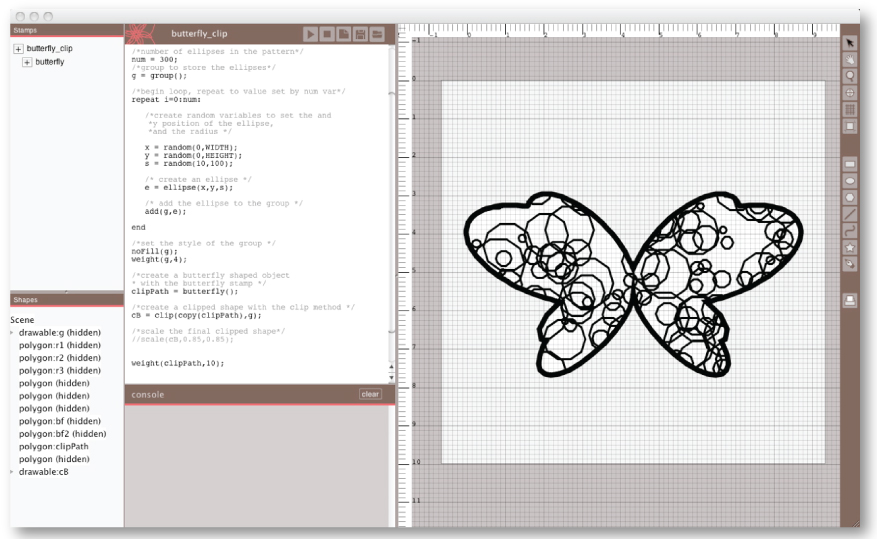
\includegraphics[width=\columnwidth]{images/dresscode_interface.jpg}
\caption{The DressCode software}
\label{fig:dresscode_interface}
\end{figure}
\end{center}
\subsection{Interface}
The interface of DressCode is divided into two sections: a design panel on the left and a coding panel on the right. The design panel contains features standard to digital graphic design software, with rulers, a grid, a drawing board, and a graphic tool menu. The drawing board defines the coordinate system referenced by the drawing API with the upper left hand corner corresponding to (0,0) in cartesian coordinates. Users can resize the drawing board and set the units to inches or millimeters by selecting the drawing board icon in the tool menu. The pan and zoom tools allow the user to navigate around the drawing board, and the print tool opens a dialog that allows the user to export their current design in vector format for output through digital fabrication. 

The coding panel contains a text editor for writing code and an output console for print output and error reporting. It also contains two additional panels, a declarative listing view, and the stamp menu, discussed in the graphic tools section. A toolbar on top of the coding panel allows the user to save their existing program, open a program, and run their current program. When a program is run, the resulting design is displayed in the design panel.

\subsection{Programming Language and Drawing API}
The DressCode programming language is interpreted with semantic functionality that is simulated through a Java-based library. For most user-defined programs, the interpretation process is instantaneous; however, some programs with complex operations require several seconds to be executed. DressCode features a custom textual programing language with native 2D drawing functionality\footnote{A full specification of the DressCode language and API is available at: \url{http://jacobsj.scripts.mit.edu/dresscode/index.php?title=Drawing_API_Reference}}. The language supports conventional programing datatypes, (numbers, strings, booleans, and lists), as well as drawing primitive datatypes, included in the drawing API. The language supports basic expressions, conditionals, loops, user-defined functions and variable assignment. Variables in DressCode are dynamically typed in order to reduce syntactic challenges for people new to textual programing and identifiers can be assigned to datatypes that differ from their original assignment at any point. The language also has built in math and random functions, including trigonometric functions, a Euclidean distance function, and three random noise generation functions: uniform, gaussian and Perlin. 

The DressCode drawing API is formulated on an Object Oriented Programming (OOP) paradigm which enables users to create geometric primitives (points, lines, curves, polygons, ellipses, rectangles and imported SVG primitives), and manipulate them as objects. Primitives are initialized by calling the appropriate method and passing it a set of parameters designating the primitive's location and dimensions. Each primitive is drawn in the design panel relative to this central origin point. There is no ``draw" method for DressCode. All primitives are automatically drawn in the order of their initialization in order to simplify the steps for a design to appear on the screen.
 
All primitives in DressCode can be modified through two kinds transformation methods, geometric and stylistic. Geometric transformations allow for primitives to be rotated, scaled, moved or combined with other primitives through polygon boolean operations, (union, intersection, either-or and difference), and are performed relative to the origin of the primitive, unless otherwise specified. A specialized boolean operation, \textit{expand},  enables the conversion of strokes to filled polygon paths, enabling the translation of line art to a form that will maintain its appearance when fabricated on a laser cutter, vinyl cutter or CNC milling machine. Stylistic transformations modify the appearance of a primitive by setting the fill and stroke color and weight, or prevent the primitive from being drawn. Transformations are performed by assigning an identifier to the primitive, and then calling the transformation method with the identifier. By using the transformation methods to manipulate primitives it is possible to generate complex and generative designs from the repetition and structured distribution of simple forms. 

As a method of organizing sets of primitives, DressCode contains a group datatype, a specialized list for organizing and performing collective transformations on multiple primitives. Groups automatically maintain an origin that is the average of all their children's origins. Groups also facilitate more advanced transformations; it is possible to clip a group of primitives within the bounds of a single primitive to serve as a form of clipping mask, and a union can automatically be performed on all objects in a group with the merge method.
 \begin{center}
\begin{figure}
\begin{lstlisting}
//repeat statement
repeat i=0:10:
ellipse(0,i*10,10,10); //draws a vertical row of 10 ellipses
end
\end{lstlisting}
%\caption{loop definitions}
%\label{fig:loops}
\end{figure}
\end{center}
We chose to create a textual programing language for DressCode because we believe textual programing is well suited to transparent representations of computational design algorithms, however we recognize that textual programing can be challenging for novices. In recognition these challenges and in a desire to extend the types of design which were possible with computational tools, we augmented the programing language with visual interaction and feedback in the form of graphic drawing tools.
 
\subsection{Graphic Tools}
\label{subsec:graphic_tools_test}
The drawing and manipulation tools in DressCode are designed to allow users to create and modify elements of their design through graphic selection. Collectively, the drawing functionality of the tools is similar to the functionality of many existing forms of  2D vector graphics software. The tools are distinguished from other graphics software tools because they maintain a direct symmetry with the DressCode programming language. Each tool correspond directly to a method in the drawing API. More importantly, the use of each tool automatically generates a corresponding textual statement in a user's program. This enables elements that are created graphically, to be immediately manipulated through textual programing, and is designed to encourage a natural flow between graphic drawing and textual programing throughout the design process. 

\begin{center}
\begin{figure}[h!]

\includegraphics[width=\columnwidth]{images/graphic_tools.jpg}
\caption{The graphic drawing and manipulation tools in DressCode (from left to right: selection and move tool, rectangle tool, ellipse tool, regular polygon tool, line tool, curve tool, SVG import tool, pen tool)}
\label{fig:graphic_tools}
\end{figure}
\end{center}

The toolset includes regular primitive creation tools (ellipse, rectangle, polygon, line curve), and an SVG import tool. There is also a pen tool that allows for the creation of irregular forms (figure:\ref{fig:graphic_tools}). Use of the pen tool generates a list of points in the text program, and statement initializing a polygon with the list. Because of the symmetry between the DressCode graphic tools and the DressCode language, there is no functionality hidden from the user in the process of modifying elements graphically. The program that results from a graphically modified design is human readable, and can be frictionlessly shared with other users or copied and pasted into other DressCode programs. In addition to the primitive generation tools, there is also a selection tool, which allows for individual primitives and groups to be manually selected with the cursor, and moved to different points on the drawing board. When a primitive is moved for the first time, a textual move statement is inserted into the user's program, with the identifier for the moved primitive as the first argument. If the moved primitive does not have an identifier, the primitive declaration is wrapped by a move statement. For all subsequent moves of that primitive with the move tool, the inserted move statement is updated to reflect the new coordinates of the primitive (figure:\ref{fig:auto_generated_code}).

\begin{center}
\begin{figure}[h!]
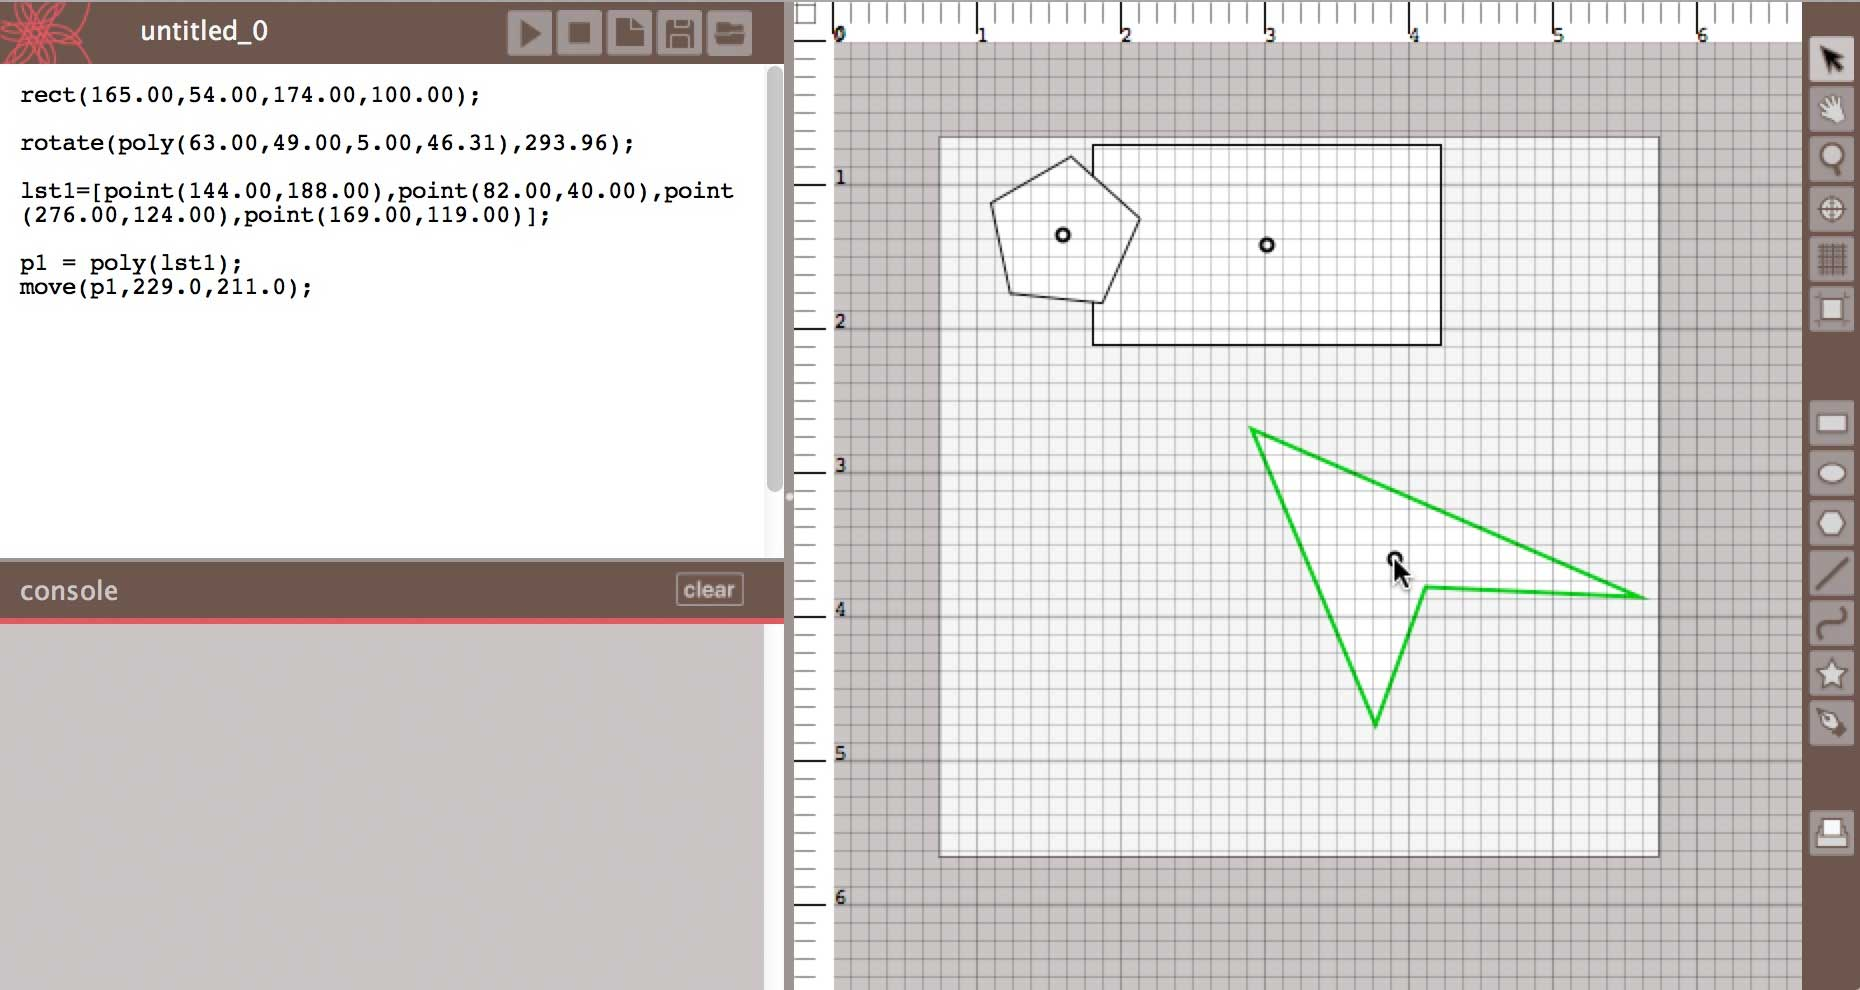
\includegraphics[width=\columnwidth]{images/auto_generated_code.jpg}
\caption{Graphically created polygon, rectangle, and irregular polygon, and corresponding automatically-generated code. (The irregular polygon has just been moved with the selection tool.)}
\label{fig:auto_generated_code}
\end{figure}
\end{center}

It is also possible to select primitives by using the declarative view panel. The declarative view contains a listing of all primitives in the current design and their type and identifier. Child primitives of groups are shown as nested elements below the group. When a primitive is selected in the declarative view, the primitive is simultaneously selected and highlighted in the design view, and the line where the primitive was last modified in the text-editor is highlighted (figure:\ref{fig:declarative_view}). The declarative is designed to provide visual feedback on how elements of a design connect to the a user's program, and provide a practical selection technique for selecting and modifying individual elements within a complex design.

\begin{center}
\begin{figure}[h!]
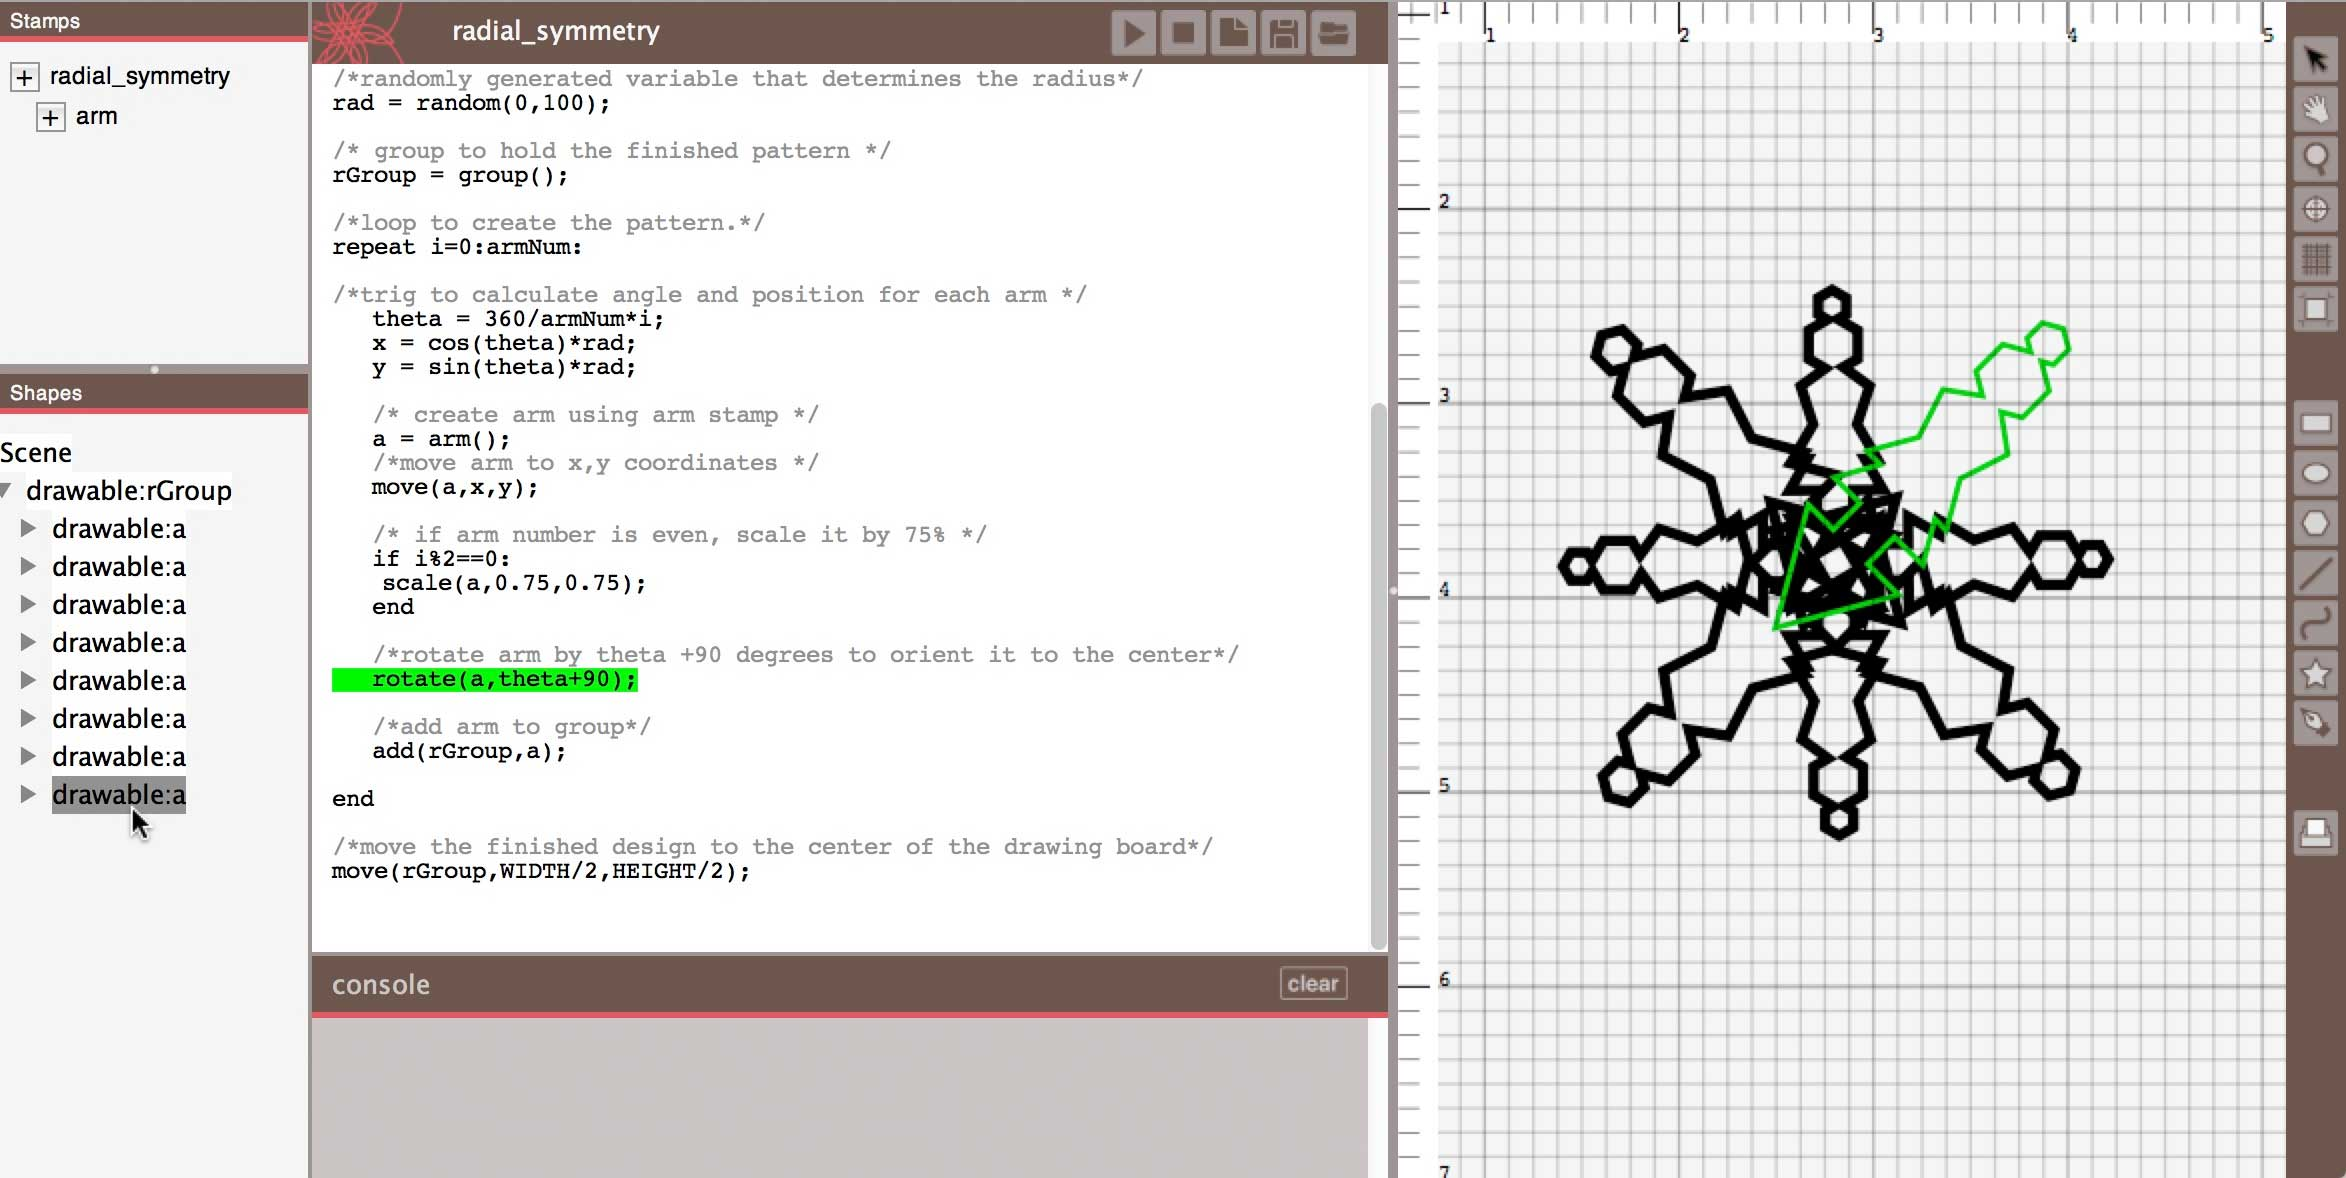
\includegraphics[width=\columnwidth]{images/selection_mechanism.jpg}
\caption{Declarative view with selected primitive}
\label{fig:declarative view}
\end{figure}
\end{center}

DressCode contains functionality to help people organize their code in the form of \textit{stamps}: graphically created functions that return shape primitives. There are two forms of stamps: dynamic and static. Dynamic stamps are created by selecting a portion of code in a user's program and then selecting the dynamic stamp option from the menu. A dynamic stamp will package the selected code in a function with a name specified by the user, and automatically return any primitives that are generated by the code in the last line of the function. Static stamps are created by graphically selecting a single primitive or group with either the selection tool or the declarative view, and selecting the static stamp option. Similar to dynamic stamps, static stamps return a copy of the primitive or group that is selected, but differ in that their code is an explicit representation of the selected primitives rather than a duplicate of the user's code. Static stamps will translate shapes generated in random positions to explicit primitives, allowing users to save a specific instances of a generative design (figure:\ref{fig:stamps}).  Stamps are listed the stamp menu and can be added to a user's primary program by selecting the \textit{+} icon next to each stamp. The code of both static and dynamic stamps can be modified by the user, by selecting the stamp from the menu, which will display the stamp code in the primary code window in an editable format. The code generated by static stamps is human readable, however if very complex designs are selected, the stamp function will consist of numerous lines of code.

\begin{center}
\begin{figure}[h!]
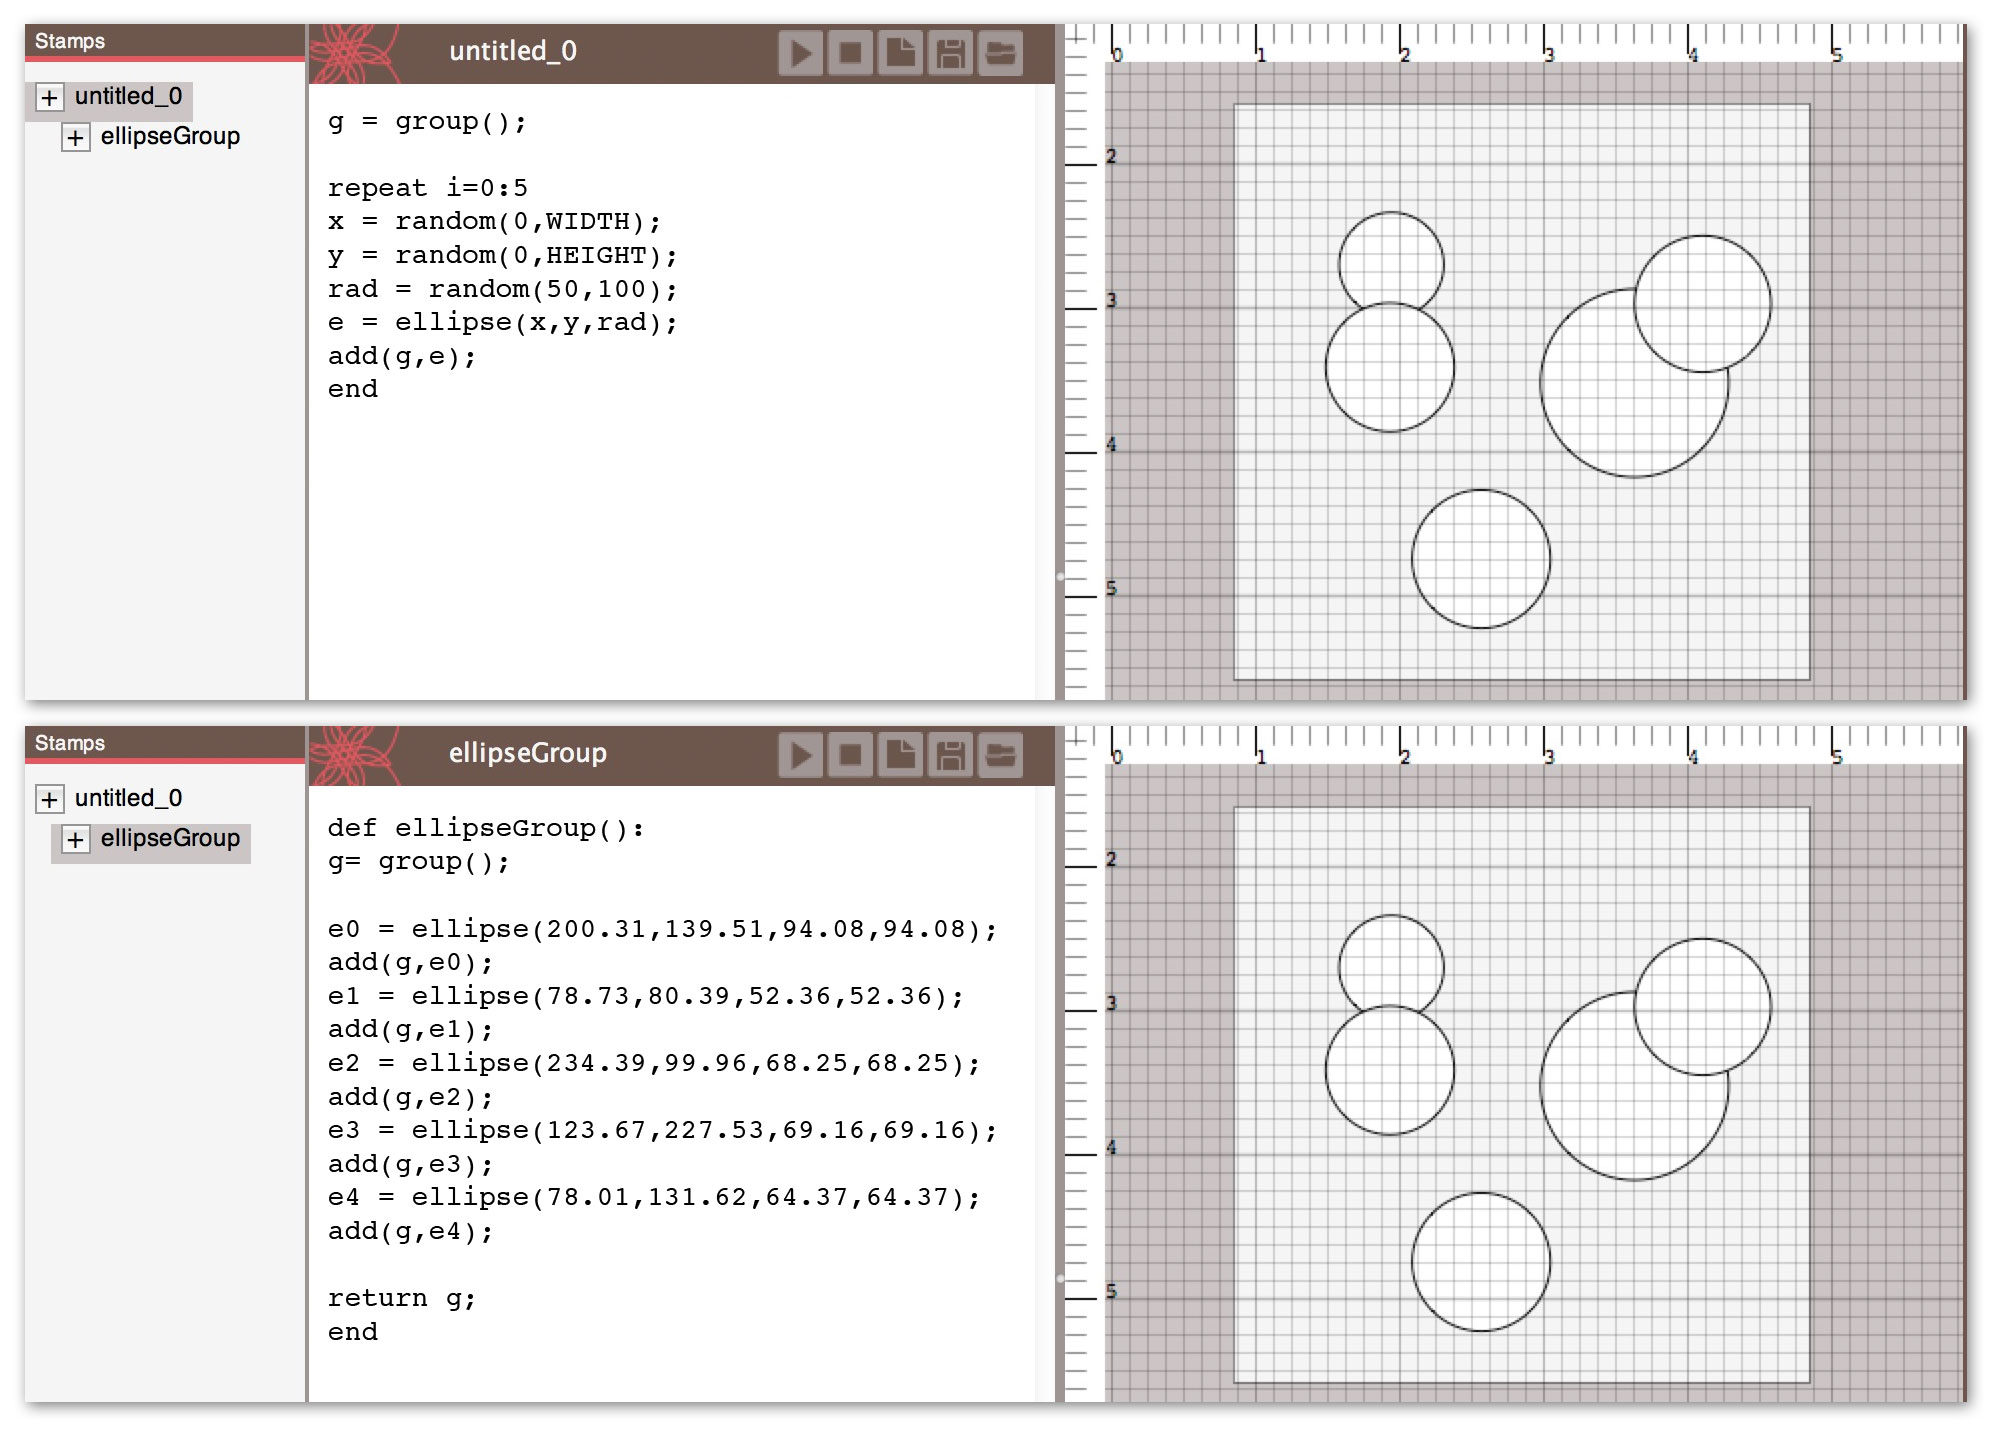
\includegraphics[width=\columnwidth]{images/stamps.jpg}
\caption{Static stamp functionality. (Top: User defined code which generates five random ellipses. The ellipses' positioning and size will change each time the program is run. Bottom: static stamp created from ellipses which will always return the same design.)}
\label{fig:stamps}
\end{figure}
\end{center}

\section{Activity Design}
Domain-specific software is an important component of engaging youth in algorithmic craft; however it is equally important to appropriately design the context in which the software is applied to the production of craft artifacts. In this section, we discuss the primary components of our activity design using DressCode: \emph{learning, creation and reflection}. These components are directly influenced by the Brennan and Resnick's dimensions of computational thinking: \emph{concepts, practices and perspectives} \cite{computational_thinking}, but are specific to algorithmic craft.

\subsection{Learning}
Learning components of activities relate to participants' understanding of the core affordances of computational design (precision, complexity, generativity, parameterization and documentation), and the values of craft (materiality, pleasure, unification of form and function and craftsmanship). Computational learning in algorithmic craft entails learning programing concepts\cite{computational_thinking}, including, sequences, data, loops, conditionals, operators and noise, and recognizing how these components relate to visual design objectives. Respectively, craft learning involves participants learning technical aspects of manual craft practices (jewelry making, screen printing, sewing), evaluating their computational designs in respect to the affordances and limits of these practices, and understanding the workflow in combining computational design and craft to produce a unified artifact. 

\subsection{Creation}
Creation components of activities emphasize practices that participants rely upon to successfully create finished algorithmic craft artifacts. Here we focus on \emph{iteration and repetition}, \emph{reusing and remixing}, and \emph{critique and debugging}. These components connect relate to Brennan's computational thinking practices, but are expanded to include mechanisms for successful craft practices. In practicing computational design, participants engage in a process of design iteration, wherein they approach a design solution through incremental steps. Iteration in the craft aspects of a project is better represented as repetition, where the objectives are simpler than in computational design objectives, but their successful execution requires repeated practice of nuanced manual skills. Reusing and remixing play key roles both in computational and craft aspects; example programs serve as starting points and references for novice designers, participants combine existing designs to produce something new, or borrow code from the designs of other participants. Parallels occur in craft, where participants duplicate and trade parts, produce multiple versions physical of a design, or incorporate found materials into their artifact.

\subsection{Extension}
Algorithimic craft activities emphasize forms of extension through \emph{reflection, sharing and connection}. Reflection occurs when participants examine what they have created and evaluate successes and challenges in its' production. Reflection is often facilitated by the process of sharing, where participants engage people outside the activity, by sharing the process behind their artifacts, and giving them as gifts. Participants also make connections with the skills, ideas and techniques they have learned with future objectives, in the form of more additional forms of computation they wish to explore, other craft and fabrication practices they want to learn, and future artifacts they plan to create. 

\section{User Study}
To better understand young people's practices in algorithmic craft, and evaluate the effectiveness of DressCode, we conducted an algorithmic craft activity using DressCode as the primary design tool. The activity consisted of a four-day workshop, divided between two consecutive weekends, in which participants created computational designs in DressCode and screen-printed them onto t-shirts.

\subsection{Evaluation Methods}
The participants' experiences were evaluated through written surveys and group discussions. Pre-workshop surveys focused on participants' previous experience and attitudes towards programing, craft and design, how personally useful they felt programing to be, and how good of a tool they found it for creativity, personal expression. They also asked students to describe their views on design, programing and craft practices as they related to referencing examples, learning from other's work. Post-workshop surveys contained attitudinal questions that were matched to the pre-surveys, as well as a range of written questions asking the participants to describe their design process, their opinion on the success of their projects and their experience using DressCode. Interim surveys were also administered following the first two days, and questioned the participants on experiences with DressCode programing language and graphic tools and how the combination of features hindered or supported the design process. We held three group discussion with the participants at the start, middle and end of the workshop which were similarly recorded and transcribed. The discussions examined participants' design process, experience using DressCode in combination with craft practices, and ideas they had for modifying or augmenting future activities and software tools. In both the interviews and discussions, participants were also asked to describe what they enjoyed, what was difficult for them, and what they felt they had learned through this process. Survey results, verbal discussion responses and project outcomes were analyzed to identify repeated and notable elements of participants experiences, and how they connected to our original research objective of helping people connect to computation in ways that are relevant, personally meaningful and intellectually engaging.

\subsection{Demographics of Participants}
The screen printing workshop was conducted among 7 young adults, aged 13-17, and one older participant, aged 21, three male, five female. Participants for the workshop were deliberately selected to represent a range of programing, craft and design experience (table \ref{table:experience}). Participants also varied on their prior experience with digital design software. Two indicated that they had no prior experience with design software, two had previously used the graphics editor in Scratch, three had used Adobe Illustrator or Photoshop, and one person was shown Solidworks in a summer course, but had limited experience with it.
\begin{table}
  \centering
  \begin{tabular}{|c|c|c|c|c|c|}
    \hline
    \multicolumn{1}{|p{0.75cm}|}{\centering\tabhead{}} &
    \multicolumn{1}{|p{1.3cm}|}{\centering\small{no experience (1)}} &
    \multicolumn{1}{|p{0.75cm}|}{\centering\small{2}}&
    \multicolumn{1}{|p{0.75cm}|}{\centering\small{3}}&
    \multicolumn{1}{|p{0.75cm}|}{\centering\small{4}}&
    \multicolumn{1}{|p{0.75cm}|}{\centering\small{expert (5)}}\\
    \hline
    \small{art} & 0 & 0 & 4 & 4 & 0\\
    \hline
    \small{craft} & 1 & 0 & 3 & 4& 0  \\
    \hline
	\small{programing} & 1 & 1 & 4 & 1& 1  \\
    \hline
	\small{design} & 0 & 2 & 3 & 3& 0  \\
    \hline
  \end{tabular}
  \caption{Prior participant experience}
\label{table:experience}
\end{table}
\subsection{Workshop Progression}
Prior to the workshop, we had participants select t-shirts in a size and color of their preference. The first session of the workshop, we introduced participants to the concept of generative design, and demonstrated techniques for incorporating random elements into a pattern or graphic. We introduced participants to textual programing in DressCode by guiding them through writing their own random walk algorithms that produced patterns composed of lines. Following this, we explained the functionality of the graphic drawing tools, and had participants modify their random walk patterns by incorporating shapes they created graphically. The following session we discussed the general process of photo-emulsion screen printing and demonstrated several other forms of generative design. We provided them with images of sample designs and had them work in groups to write a set of instructions that they thought would re-produce that design. As a group we discussed their results, and then demonstrated examples in DressCode that would produce similar results to the sample designs (figure:\ref{fig:example_designs}). 
\begin{center}
\begin{figure}[h!]
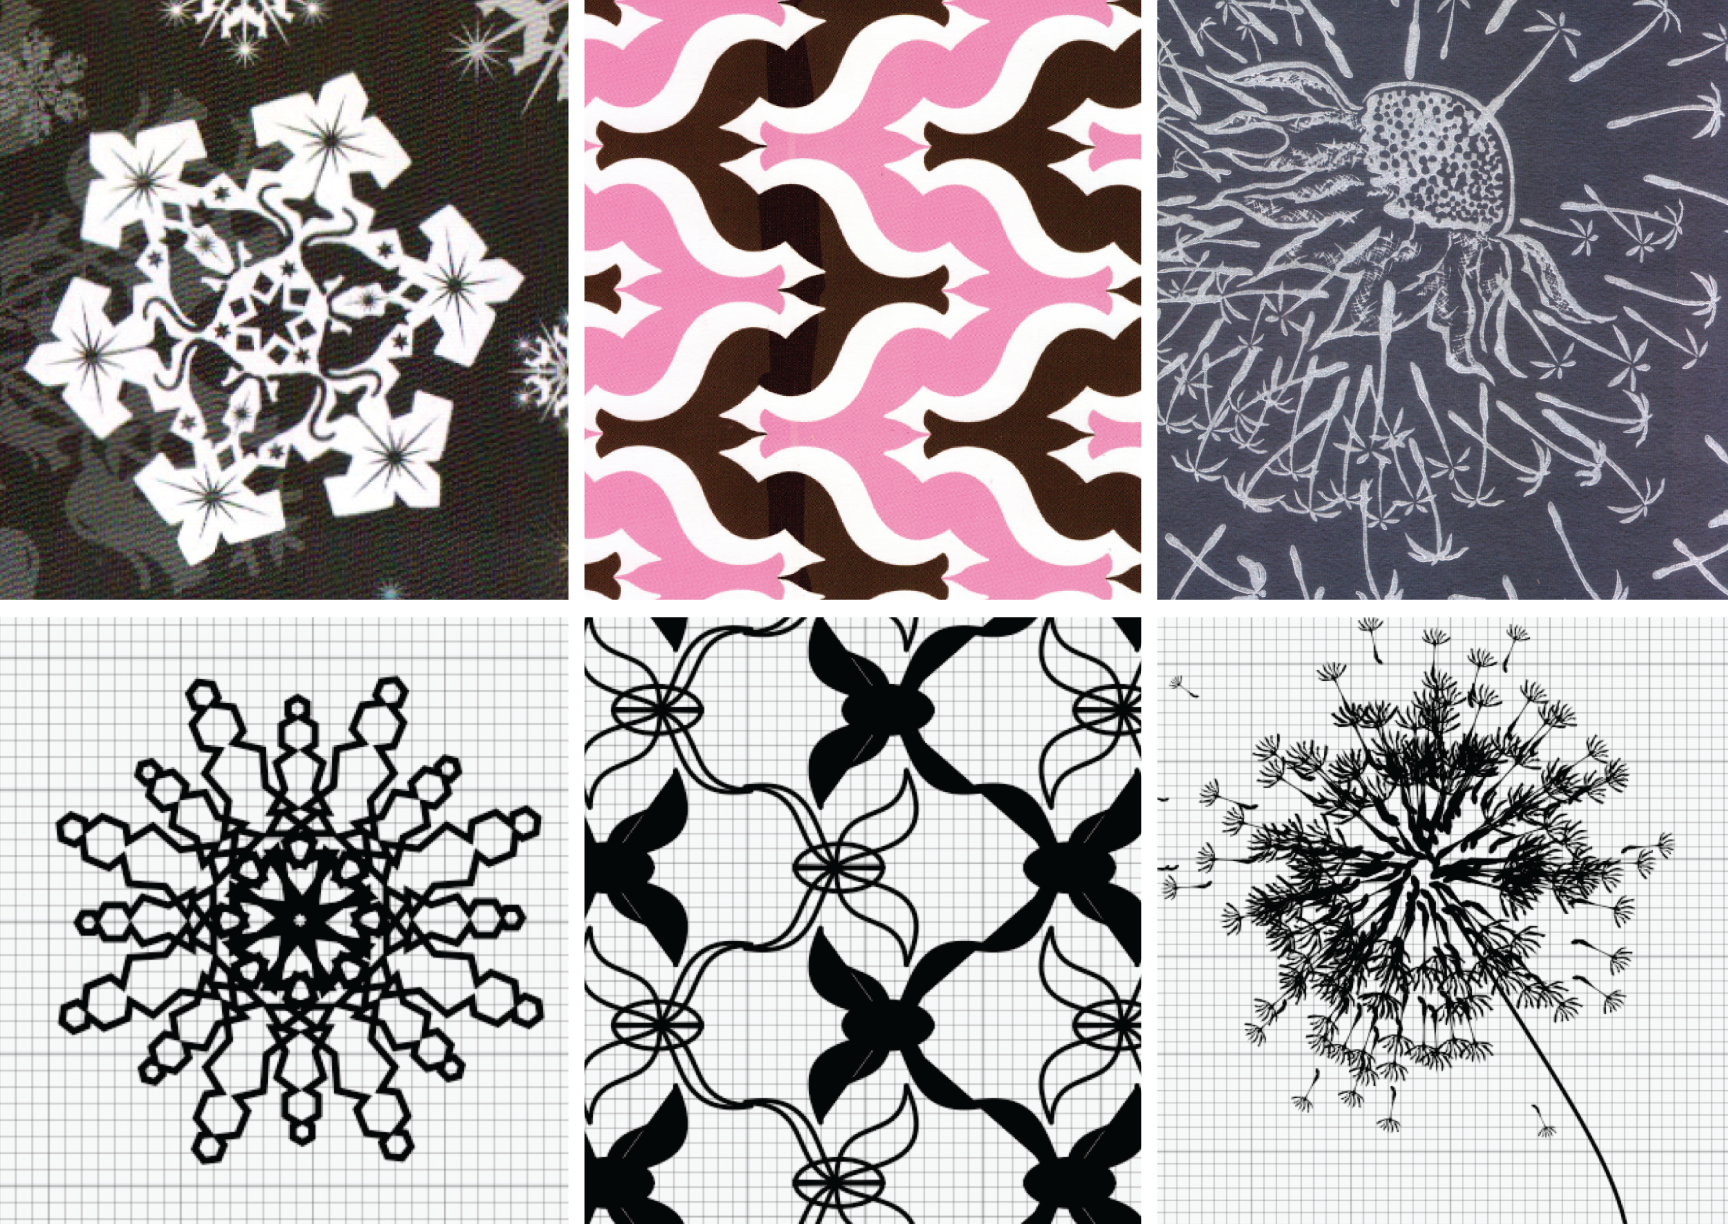
\includegraphics[width=\columnwidth]{images/pattern_examples.png}
\caption{Sample designs and corresponding examples in DressCode}
\label{fig:example_designs}
\end{figure}
\end{center}
Participants were then provided with the design task of creating a computational design to screen print onto a t-shirt they would want to wear, and given 3 hours of open design time with the option of modifying the examples we provided, working off of the original random walk pattern they had created the first day, generating a design from scratch, or working with an instructor to come up with additional design ideas. The following session participants prepared their screens for screen printing, by stretching the screen material over the frames in groups and applying the photo emulsion to their screens. Afterwards, participants were given 2.5 hours of additional open time to complete their designs. Participants laser-printed their finished designs on transparencies, which the instructors exposed on the screens overnight (figure:\ref{fig:screen_printing_process}). The final session, participants practiced printing with their designs on test materials, and then printed onto their t-shirts.
\begin{center}
\begin{figure}[h!]
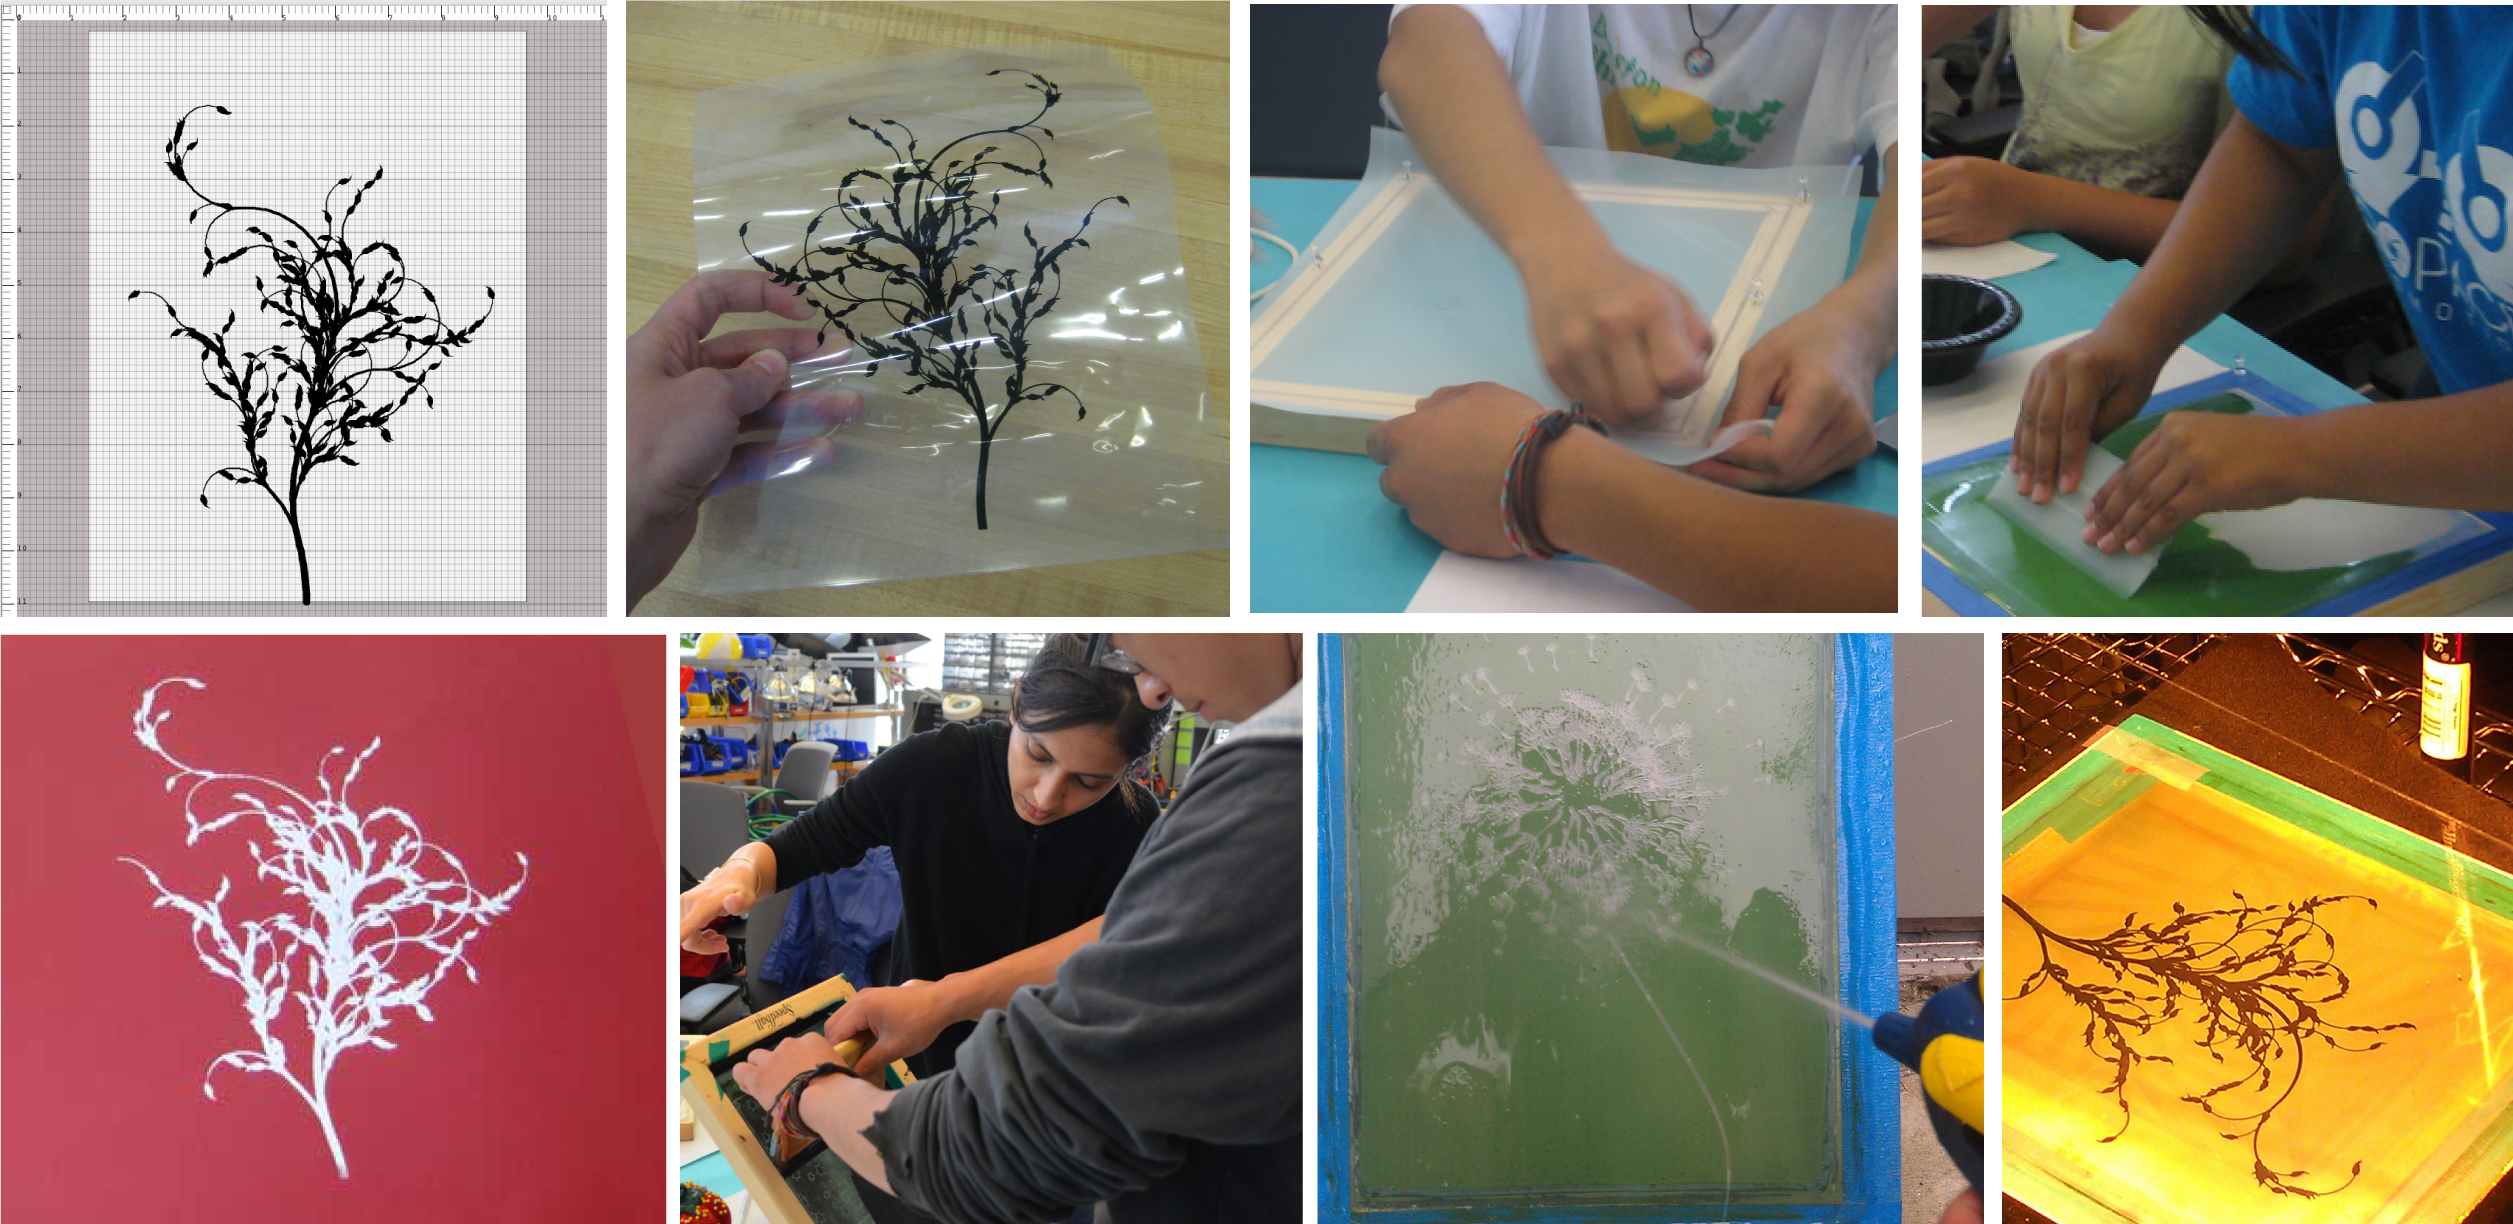
\includegraphics[width=\columnwidth]{images/screen_printing_process.png}
\caption{Screen printing process. (Clockwise from upper-left: Digital design, printed transparency of design, stretching the screen, applying photo emulsion, exposing the screen with the transparency, washing out the screen to reveal the design, printing with the finished screen, a completed print.) }
\label{fig:screen_printing_process}
\end{figure}
\end{center}

\subsection{Screen Printing Results}
Each participant in the primary workshop was successfully able to use DressCode to produce a design for their t-shirt (figure \ref{fig:screen_results}). The design approaches among the participants varied. Two participants created designs that were derived from their random walk algorithms, one participant created a pattern by combining two of the example patterns and making adjustments, and one participant worked solely by modifying an example. Other participants designed patterns independent of the examples, including a generative landscape, a geometric spiraling pattern and a complex radial pattern comprised of overlapping lines. Discuss importance of booleans. The screen printing process was extremely popular among the participants. Each person was successful in creating their screen, transferring their design to the screen and printing to the shirt, although one participant had to re-expose his screen because of errors in applying the emulsion. Several participants not only printed to the provided shirts, but also brought in additional garments to print on for friends and family. The participants requested to keep their screens following the workshop, and stated on the survey that they planned to continue making prints for themselves and others. All participants indicated that they planned to wear their shirts, and two participants contacted us via email following the workshop thanking us for the experience, and requesting tips on how to properly care for their garments. 

\begin{center}
\begin{figure}[h!]
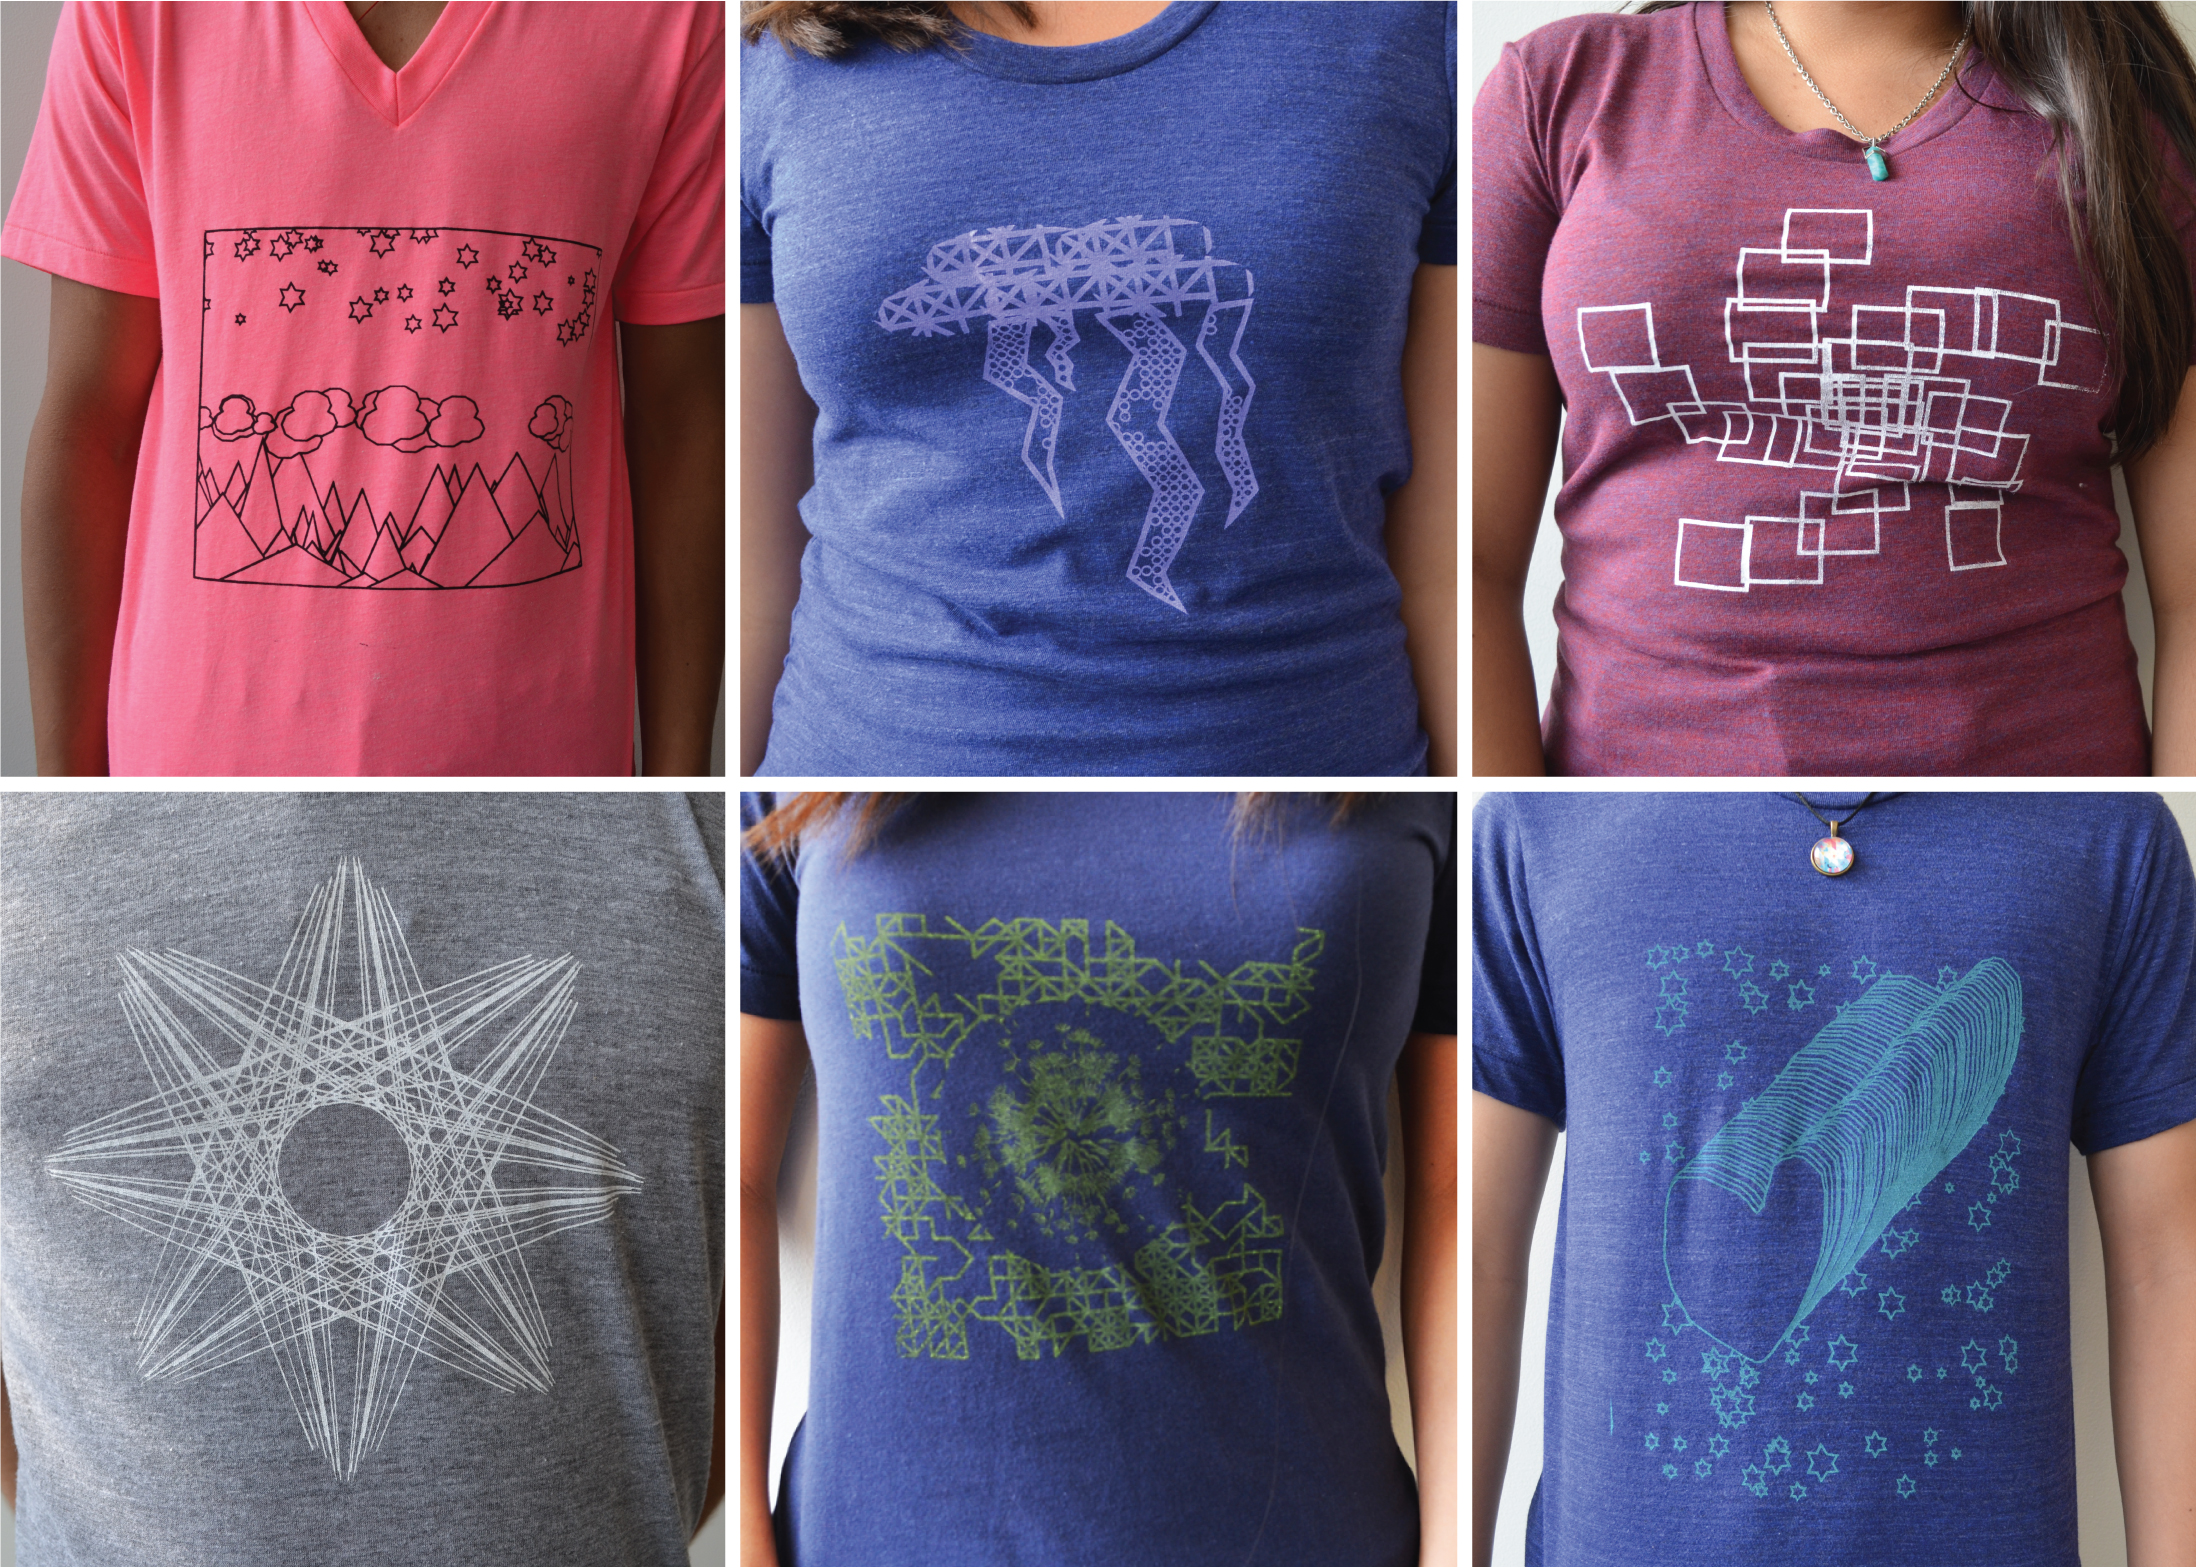
\includegraphics[width=\columnwidth]{images/shirt_results.jpg}
\caption{Completed shirts from screen printing workshop}
\label{fig:screen_results}
\end{figure}
\end{center}

From survey data and group discussions, 3 participants found the screen printing portion to be most difficult, 3 found the programing to be the most difficult, and one was equally challenged by both portions. An evaluation of the pre, mid and post-workshop surveys demonstrated that following the screen printing, participants attitudes towards programing, design and craft, changed from what they were after the computational design sessions. In the majority of cases, this change was positive; participants indicated greater interest in learning programing in the future, a stronger belief that programing was a tool that they could create things they would use in their daily life, and greater comfort in programing on their own following the craft activity. Six of the eight participants stated that they liked their design better after printing it, and all participants stated that the process of screen printing had given them ideas for additional designs they would like to create with DressCode. For a minority of participants however, the difficulty of the craft portion seemed to result in a slightly diminished interest in combining craft and programing, and a diminished interest in craft in general. Participants were positive about the graphic tools, although they requested that their functionality be extended to incorporate a greater range of transformation methods (rotation, scaling, and boolean operations). All 8 participants said they would be interested in using DressCode for another activity, and the majority indicated that they would like to combine computational design with 3D printing, and 7 of 8 participants indicated they would like to continue using the programing language in particular.

\section{Discussion}
In our discussion of the workshops we focus on three primary elements of the participants' experiences. First, we examine the successes and limits of the DressCode software, with an emphasis how people used the graphic drawing and manipulation functionality. Second, we evaluate participant's design practices and discuss how they connect to the  affordances algorithmic craft. Finally we consider what participants got out of the workshop, by describing participant reactions to their finished artifacts and evaluating how these artifacts resonate with participants' personal values and daily lives.

\subsection{Design Principles for Combining Graphic Manipulation with Textual Programing}
	One of our primary research objectives was to develop techniques that were accessible while also supporting personal aesthetics and styles through computational design. Analysis of participants' use of DressCode indicates that for many people, the graphic tools were helpful in this regard. The graphic drawing tools were used in the majority of participants' designs (table \ref{table:graphic_tools}. 

\begin{table}
  \centering
  \begin{tabular}{|c|c|c|c|c|c|}
    \hline
    \multicolumn{1}{|p{0.75cm}|}{\centering\tabhead{}} &
    \multicolumn{1}{|p{1cm}|}{\centering\small{str. disagree}} &
    \multicolumn{1}{|p{0.8cm}|}{\centering\small{disagree}}&
    \multicolumn{1}{|p{0.8cm}|}{\centering\small{neutral}}&
    \multicolumn{1}{|p{0.8cm}|}{\centering\small{agree}}&
    \multicolumn{1}{|p{0.8cm}|}{\centering\small{str. agree}}\\
    \hline
    \small{helped create design} & 0 & 1 & 1 & 3 & 2 \\
    \hline
    \small{helped understand program} & 0 & 0 & 5 & 3& 0  \\
    \hline
  \end{tabular}
  \caption{participant survey responses on the role of graphic tools}
\label{table:graphic_tools}
\end{table}

Participant responses on the survey and during discussion suggest the tools were accessible to use, and assisted many in understanding the functionality of their programs. Before the graphic tools were formally introduced, several participants independently started experimenting with them on their own. Several people also indicated that the graphic drawing tools also helped them to better understand the process of writing their program. Participants expanded on this idea during the discussion:
\begin{quotation}
\textit{I think that the way it already is, is pretty good. You find a tool, you draw on the canvas and it shows you the code, that's basically it.}
\\Participant Z
\end{quotation}

\begin{quotation}
\textit{I think that having the drawing tools and having it also show the code there makes it so that you can see as you're doing it, like if you make a line from this point to this point to this point this is actually what the code is doing, so having a graphical side and having it auto update the code, and so it can show you that you want to work with the code you're learning as you're using the GUI too. So that people could try and say ok, if I can't do something with the graphical tools, let me try and manipulate the code. And then you already have some understanding because you've been using the graphical tools and it's been appearing over there the entire time.}
\\Participant B
\end{quotation}

A visual examination of many of the finished products in the workshop demonstrates the impact the graphic drawing tools on the aesthetics of the designs themselves. The pen, and shape generation tools allowed participants to blend their personal drawing styles with computational elements, resulting in computational forms that reflected the drawing techniques of the creator. 

%put in image of heart and cloud

Beyond facilitating the design process, the introduction of the graphic tools also resulted in a discussion among participants in the primary workshop about future paradigms for graphic design and programing tools. This discussion pointed to specific elements in the graphic tools that participants found confusing or helpful. Participants were unanimously agreed on the utility of the drawing tools, but requested that they be developed further to provide more sophisticated forms of drawing, control, and visual feedback. Incorporation of more sophisticated drawing tools would provide the opportunity for further personalization of computational forms.

While the primitive drawing tools proved to be popular among the participants, several had difficulty with the move tool. From a development perspective, the move tool was challenging to implement because there were numerous possibilities on how it could be represented in the user's code. We implemented what we felt to be the simplest option (inserting a move statement for primitives with identifiers, or wrapping the declaration statement of un-identified primitives), but doing so required us to speculate about what would be most useful and intuitive for novice programmers. In practice, participants who had large numbers of primitives in their programs without identifiers found the move tool behavior confusing because it modified an existing statement in their program, rather than generating a new line of code. This frequently resulted in syntax errors when the participant then modified shape statement and omitted a parentheses or placed arguments in the incorrect portion of the statement. These issues make it clear that we should re-consider the functionality of the tool, however they also convey a general design principle for future tools. The fewer assumptions a tool has to make about the intentions of the user, the less likely it is that it will conflict with the user's coding and design process. Furthermore, the fewer the assumptions, the easier the tool will be to implement. We feel the creation of more sophisticated primitive generation tools is a form of low hanging fruit that will provide immediate benefits to the user's design process, whereas transformation tools require greater analysis on how to be implemented effectively. Participants responses in the discussion also demonstrated ways in which the tools had expanded their comprehension of the computational design process. One participant suggested adding an graphic erasing tool, which resulted in a conversation on how such a tool could be implemented:

\begin{quotation}
Participant M: \textit{[I want] an erasing tool, so you can erase the line kind of like in Sketchup.}  
Participant Z: \textit{So if you erase one line, it becomes two lines...so it's going to generate the code for two lines?}
Participant M: \textit{No like if you drew a line with the sidebar, and then you decided you didn't like, you don't have to go to the code, erase it and press play, you could just take the erase tool, click on it and then it goes away.}
Participant Z:  \textit{No, what I mean is like if you just wanted to erase half?}
Participant M: \textit{Or you could just drag the shapes and it just goes away.}
\end{quotation}

This conversation reinforces the difficulty in making assumptions about individuals' design processes in the implementation of graphic tools. Moreover, this discussion shows the participants actively considering how new graphic tools could correspond to writing code. Conversations of this nature demonstrate how graphic tools can stimulate thinking about computational processes for young programmers, rather than making them opaque. During the workshop, a similar discussion occurred around the topic of preserving generative forms. Participants had different ideas for how they would wanted to preserve static instances of randomly generated designs. Several participants used the static stamp tool for its intended purpose during the workshop, but others requested different forms of control over the randomly generated values. One participant wondered if they could have the software store the randomly created values for a specific program, and allow the user to specify the point at which new values would be generated. Building on this idea, we asked participants if they would have preferred to specify random and noise generation through a form of graphic input similar to the graphic dialog tools, or if they felt creating random methods in the programing environment was useful. Two participants said they would prefer that as an option, however others disagreed, stating that they felt you would lose some of the functionality of the program in the process.
\begin{quotation} 
\textit{Well that would kind of take away from the programing part of it, because you'd be trying to turn everything into a UI.
The important thing I really feel about DressCode is you can turn things like random, these are drawn (indicating a hand drawn graphic) and these are from the programing part (indicating the random repetition of the graphic), but in Illustrator it's just drawing, you can't have everything.}
\\Participant Z
\end{quotation}

Understanding the creative potential of one's tools is essential for effective design. It is encouraging therefore, that many participants not only saw the value of the graphic tools, but also understood and embraced the applications of textual programming in combination with these tools. 

The introduction of graphic manipulation tools in conjunction with textual programing demonstrated several conclusions. Drawing tools proved to be largely intuitive and easy to use and they distinguished the participants' designs from one another, and from the work of participants in the prior workshop without the tools. The incorporation of personal drawing styles techniques is highly relevant to our objectives in algorithmic craft, because it allows people create artifacts that are personally unique, and conform to the stylistic preferences of the individual who produced them. Furthermore, the evaluation of the tools by the participants demonstrated that the tools were assisted in communicating basic computational principles as demonstrated by participants description of how they would want additional tools to function. Lastly, despite participant's requests for more sophisticated forms of transformation tools, we feel their implementation should be tempered by careful consideration of a successful design strategy for integrating them with the process of programing. 

\subsection{Algorithmic Crafting in Practice}
\textbf{what did people actually end up doing?}
If the graphic tools assisted with some of the technical challenges of algorithmic craft, we are still left with the questions regarding the actual practice of algorithmic craft. How did the experience affect participants perceptions towards computation and craft? Were individuals able to take advantages of computational design affordances in ways that connected to their personal design goals? What effect did our feedback mechanisms have on the success of people's projects? We begin our discussion of these components by describing changes in participants' perception. 

Following the workshop, participants displayed an increased awareness of the design applications of programing. 
\begin{quotation}
		\textit{I never thought of using programming as a tool to help create a design. There are so many things you can design using programming languages.}
		\\Participant R
		
		\textit{I now know that there are so many more possibilities of programming because I've seen a connection.}
		\\Participant J
		
		\textit{When I got the hang of [DressCode], I loved how much you could do with it. There's such a broad range of design possibilities, and with every new one you create, you learn more about the various tools and become more familiarized with DressCode.}
		\\Participant E
\end{quotation}

More importantly, the participants demonstrated a nuanced understanding of the process of designing itself, and carefully considered how computation could play a role. 
\begin{quotation}
	\textit{Before I thought that design was relatively simple, but now I see that a lot of thought has to go into what you're making and the process of how to make it.}
		\\Participant E
	\end{quotation}

\begin{quotation}
	\textit{I've learned new controls like the random code and it's really just small steps and things I learn through DressCode that allow me to fully express my creative side and expand my knowledge of design.}
	\\Participant J
\end{quotation}

A general perception of the applicability of programing to design is a fundamental step to participating in algorithmic craft. It is more challenging however for people to understand the specific affordances of computational design and incorporate them in their practice. The participants in the screen printing workshop performed even better than we hoped in this respect. A combined evaluation of their end products, and statements from the discussions and surveys points to the clear presence of the principles of computational design. When asked how using DressCode had changed his creative process, one participant responded that he was trying out ideas that were similar to work he had created before the workshop, but now had the opportunity to execute them with greater \textit{precision}. Another participant described her design process this way:
\begin{quotation}
	\textit{It's very different- I draw everything, and I never could've created my design by hand.}
	\\Participant J
\end{quotation}

Her description of her process, like her design itself \ref{emily_design} revolves around the idea of the \textit{visual complexity} that is enabled through computational iteration and repetition. Her design is also an example of \textit{remixing}, as she combined portions of the code from an example with a program she had written herself, making adjustments to both to produce a novel composition. Another participant incorporated aspects of a fellow participant's program into his own design by adding the code for the stars in the landscape design to his heart design. The landscape design serves as an example of the benefits of parameterization. In the last five minutes of the design session, the participant decided that a horizontal composition would look better on his t-shirt than a vertical one. Because he had defined variables for the random distribution of clouds, mountains and stars that corresponded to the width and height of the drawing board, when he resized his drawing board, the design was automatically re-generated to correspond to the new size. The participant stated in the survey that:
\begin{quotation}
	\textit{[DressCode] made changes much easier to change, rather than redoing the entire design}
	\\Participant R
\end{quotation}
Generativity played a role in the majority of participants designs. All but two of them incorporated some form of noise in their code. Below, a participant with no prior programing experience describes her experience in using uniform noise in her design:
\begin{quotation}
	\textit{The random thing.. if you made it random by hand then it wouldn't really be random, because you would just put it in a special place.. so the computer just has to choose where to put it.}
		\\Participant M
\end{quotation}
The participant who created the randomized radial pattern was demonstrated the most elaborate use of generative design in the workshop. During the second critique, he presented 17 unique and complex patterns, solely comprised of overlapping lines. This astonished the other participants who were surprised to see that such variety could be produced by one algorithm. He described his process with DressCode in this way:
\begin{quotation} [DressCode] allowed me to see random patterns such as the one I made. I may have been able to otherwise, but I probably wouldn't have thought to.
		\\Participant B
	\end{quotation}

Aside from implementing specific affordances of computational design, participants also ran in to challenges that are particular to computational design. 
One participant used gaussian noise to distribute elements of her design, but wanted to deviate from this structure at several key instances to produce an emphasis in her composition. In attempting to do so however, she struggled in determining how to have her algorithm deviate from the gaussian distribution and arbitrary points. Her struggles touch upon the larger challenge in computational design of creating singularities. Because computational design is governed by a systematized ruleset, the methods of breaking these rules at arbitrary points are often unclear or tedious to implement. Another challenge in computational design involves the process of formalizing complex problems. As design problems grow in complexity, formalizing the problem in a manner that can be expressed programmatically becomes increasingly difficult. The participant who created the generative landscape pattern wished to modify his design so that the distribution of the mountains, clouds and stars appeared more ``realistic''. He had difficulty reconciling his intuitive understanding of the qualities realistic landscapes with a set of formal properties that could be communicated through programing. Lastly, the the participant who created 17 instances of his design was challenged when it was time to choose a single instance to screen print with. Computational design gives the designer the ability to produce extremely large numbers of solutions to a single design problem. While this is useful in situations where multiple solutions are required, when a single design must be chosen, the process of deciding on a solution is difficult, especially if the decision is based on aesthetic criteria.

The challenges participants encountered in the design process were addressed primarily through two forms, individual instructor assistance and group critiques. Although instructor assistance was important to the success of the workshop, in many ways it mirrored instructor help in a general programing context and consisted of helping to correct syntax errors and pointing participants towards relevant programing methods. Here, we focus on the group critiques as the most interesting and novel form of design feedback that occurred in the workshop. As we explained to participants, in design critiques, the role of the group is to understand the creative goal of the designer, and offer advice on how they can reach that goal. Prior to the workshop, most participants had not participated in design critiques, and they were hesitant to criticize the work of their peers or offer suggestions. Through successive critique sessions participants gradually became more comfortable in voicing their opinions. By the end of the workshop, several participants stated that the critiques had helped to improve their design. For example:
\begin{quotation}
	I started with a design I was ok with, but group critique and getting others' opinions helped me create a design I loved.
	\\Participant E
\end{quotation}

During the critiques, designs were collectively ``debugged'' by the group. Feedback was often simultaneously provided in the form of stylistic suggestions and technical tips on how modify the code of a design to achieve the stylistic goal. In one instance, a participant noticed that the linear spiral pattern we were critiquing came close to producing a Moiré effect. The designer said that she had noticed the effect too, and wished to make it more apparent. As she demonstrated the code used to  create the pattern, and other participants began suggesting values she could modify to change the density of the lines and produce a more intense effect. Debugging often occurred in a craft context as well. When critiquing a design, participants considered the material limitations of screen printing, and offered suggestions on how to make a design correspond to these factors.

Group critiques also applied well to the challenge of generative design selection. The critique provided the participant with 20 design instances with the opportunity to receive group suggestions on what his final design should be, while simultaneously stimulating a discussion on the challenges of generatively among the participants. Critiques in the workshop ended up serving a purpose beyond optimizing the designs of the participants. In the process of critiquing others' work, participants \emph{learned} from their peers about the computational approaches behind their designs, and \emph{thought about} the challenges and opportunities of this form of making.

As a whole, the workshop changed participants's perceptions of the creative affordances of programing by allowing them to produce their own computational designs. Through the production of these designs, participants demonstrated both the application and understanding of key computational design affordances. Finally, group critiques helped people to improve their designs, enabled them to learn from peers about computational processes, and provided the opportunity for intellectual discussion on the advantages and challenges of computational design in general.

\subsection{Physical and Digital Notions of Value}
\textbf{what mattered to people in the end?}
\textcolor{red}{This section is not done.}
Participants varied in both workshops on the elements of algorithmic craft they found to be the most difficult, as well as the parts they found most enjoyable. People in the bracelet workshop were unanimous in their identification of the programing component as the component that they found most frustrating.
 
In comparison, the screen printing participants also found aspects of the programing challenging, but expressed a greater variety of between what they found to be difficult. Two people said the actual process of coding was most difficult, and another said that the process of understanding the concept behind her design was challenging. The remainder of the participants identified aspects of screen printing as the most challenging portion, such as preparing the screen, avoiding alignment issues, or printing without error.

Screen printing, the first print had too little ink, the next one too much, and the third one came out and that was on my t-shirt so that was good.
Miriam: The hardest part for me was actually putting the design from my screen onto any material. I had to make like 10 copies before I put it on the shirt. But yeah, I had to make a lot of copies. 
Beckett: I enjoyed the design/ creation process, but the printing itself? no
Roger: I enjoyed being able to do things myself and get help when I needed. I found it frustrating how my screen printing kept on fading

%vs first workshop where people consistently found programing portion to be difficult
%their perception of difficulty of programing increased following the workshop, but their desire to learn programing also increased directly following either the programming or craft portions.
Added value as the result of physical labor.
Does the difficulty of screen printing change how you feel about the piece
Roger: It lets you take pride in it.
Luisa: After all this hard work, you have this	

Is that similar to the difficulty of programing
I feel as though maybe like when you're programing stuff, you're on the computer but you're not using any physical work, but when you're screen printing there's the manual labor involved, so when you actually get something right it's I guess more gratifying, since you put like hard work, well you do put hard work into programing, but it's more a thinking thing, besides actual physical labor.

subsubsection{Craft and Computational Compatibility}
All participants felt computational and screen printing worked well together
All participants said that after screen printing they were more interested in computational design
All participants stated that they would like to use computational design for screen printing in the future.
All participants indicated that screen printing gave them additional ideas for things they would like to create with DressCode
All participants felt DressCode worked well with screen printing
Consideration of materials in design

Personal Accomplishment
Uniqueness

\subsubsection{Personal and Cultural Relevance in Algorithmic Craft}

cultural appropriateness of aesthetics (gender, youth)\\

entrepreneurship
Open question of what the resultant product is. (screen? artifact? program?)
Community Setting\\
 \begin{quotation}
\textit{I enjoyed the people who participated in the program because they make the whole process really fun. I love the environment we worked in, everything around us is so fascinating.}
\\Participant J
\end{quotation}

Isolation\\
 \begin{quotation}
\textit{Something I found really challenging was that many of the other participants already have lots more experience in this field than me so I kind of feel isolated and behind everyone else.}
\\Participant J
\end{quotation}


\section{Recommendations for the Design of Future Algorithmic Craft Tools and Activities}
Based on our evaluation of the workshop, we conclude with a set of recommendations for future work in developing activities and tools for algorithmic craft. 

\begin{itemize}
\item \textbf{Tools should support design techniques that demonstrate the benefits of computational design.} Tools for algorithmic crafting should effectively communicate the affordances of computational design in ways that are accessible to new programmers by providing programming examples that suggest design approaches or by creating built in functionality with compelling aesthetic potential.

\item \textbf{Programming languages should be augmented with visual feedback and intuitive drawing methods to support multiple forms of creation.} Algorithmic crafting tools should have a programming syntax and API that is designed to accommodate individuals with no prior programming experience, rather than rely on a general-purpose programming language. The API should be limited to methods and structures relevant to the task of design. By providing users with a small set of useful programming methods that can be used to generate complex forms and patterns, it becomes feasible for novices to engage in intentional and independent computational design.

\item \textbf{Tools should be supported through fabrication and craft-specific documentation.} In addition to the documentation of the application and programming language, the fabrication and crafting techniques intended for use with the software should be well-documented. This documentation should include an explanation of suitable materials, advice on digital fabrication access, specifications on machine use and settings, and tutorials describing craft components of example projects.

\item \textbf{Activities should encourage discussion and group critiques of work, and when possible, use in-person facilitation and guidance.} Algorithmic craft is a creative practice, not a technical exercise, and as such, it benefits from discussion among peers, critique, and reflection. With novice programmers, engagement in these reflective practices is best conducted in a group setting with some form of facilitation. Group algorithmic crafting activities can also provide a casual social atmosphere that is conducive to hand-craft.

\item \textbf{Activities should blend domain specificity with creative openness.} Algorithmic craft tools should be able to support numerous creative applications which will encourage the creation of personally relevant, aesthetic outcomes. To encourage the creation of personally relevant aesthetics algorithmic craft tools should be open enough to support numerous creative applications. Algorithmic craft tools should be introduced in a way that provides users with a compelling motivation for their use.

%\item \textbf{Select approaches with Craft and Computational Resonance} %ie screen printing and computational t-shirt design

\item \textbf{Materials matter.} The use of rich, interesting materials greatly enriches the experience of algorithmic craft and contributes to the success of the finished artifacts. Raw materials like leather, wood, textiles, and art-quality paper complement the precision and complexity of computational design and digital fabrication. Combined in the hands of an engaged user, they can result in objects that are attractive and durable. Care should also be taken to demonstrate construction techniques that will hold up over time.

\item \textbf{Consider the cultural implications of algorithmic craft experiences.} Because algorithmic craft can provide a form of self expression and communication, activities should aim to be mindful of the gender, age, cultural background, and social norms for participants. It is useful to engage with participants in a dialog about these topics and how they could be further supported in future algorithmic crafting experiences.
\end{itemize}


\balance

% REFERENCES FORMAT
% References must be the same font size as other body text.

\bibliographystyle{acm-sigchi}
\bibliography{dresscode}
\end{document}
